\documentclass[12pt]{article}
\usepackage[left=3cm, right=3cm, bottom=2.5cm, top=2.5cm]{geometry}
\usepackage{setspace}
\usepackage[T1]{fontenc}
\usepackage{times}
\usepackage{booktabs}
\usepackage{rotating}
\usepackage{graphicx}
\usepackage[section]{placeins} %Placeins.sty keeps floats `in their place', preventing them from floating past a "\FloatBarrier" command into another section.  To use it, declare "\usepackage{placeins}" and insert "\FloatBarrier" at places that floats should not move past, perhaps at every "\section".  
\usepackage[large, bf]{caption}
\usepackage[FIGTOPCAP]{subfigure}
\usepackage{pdfpages}
\usepackage{palatino}
\usepackage{pdflscape}
\usepackage{textcomp}
\usepackage{longtable}
\usepackage{nicefrac}
\usepackage{adjustbox}	% to adjust the size of objects to fit into a page
\usepackage[hyphens]{url}


% Citing 
%\usepackage{natbib}
%\bibpunct{(}{)}{;}{a}{,}{,}

%\def\citeapos#1{\citeauthor{#1}'s (\citeyear{#1})}


%% Citing with footnotes
% replace \cite with \autocite (and vice versa if we want to go back to apalike eferences
%\usepackage[style=verbose,backend=bibtex]{biblatex}
\usepackage[notes, backend=biber]{biblatex-chicago}
\bibliography{references}


%zero spacing between references
%\usepackage{bibspacing}
%\setlength{\bibspacing}{\baselineskip}

%%-----------------------------------------------------------------
%%Header
%\usepackage{fancyhdr}
%\fancyhf{}
%\fancyhead[C]{\textit{Preliminary and Incomplete}}
%\fancyfoot[C]{\thepage}
%\renewcommand\headrulewidth{0pt}
%\pagestyle{fancy}
%%-----------------------------------------------------------------

%\onehalfspacing
%\doublespacing

\usepackage{amsmath, amsfonts, amssymb, amsthm}

\usepackage{mathpazo} %Use Palotino fonts
\parskip 0ex  %Vertical distance between paragraphs, in "ex"s
\parindent 20pt

%\usepackage{harvard}
%\bibliographystyle{apsr}
%\bibliographystyle{dcu}

\usepackage[pdftex]{hyperref}
\hypersetup{colorlinks, citecolor=black, filecolor=blue, linkcolor=blue, urlcolor=blue}

%\makeatletter
%\renewcommand{\subsubsection}{\@startsection
%{subsubsection} %the name
%{4} %the level
%{0pt} %the indent 
%{1ex} %the before skip
%{1ex} %the after skip
%{\itshape}}
%\makeatother

\newtheorem{theorem}{Theorem}
\newtheorem{lemma}{Lemma}
\newtheorem{proposition}{Proposition}
\newtheorem{corollary}{Corollary}
\newtheorem{prediction}{Prediction}
\newtheorem{case}{Special Case}

\newenvironment{proofAlt}[1][Proof]{\begin{trivlist}
\item[\hskip \labelsep {\bfseries #1}]}{\end{trivlist}}
\newenvironment{definition}[1][Definition]{\begin{trivlist}
\item[\hskip \labelsep {\bfseries #1}]}{\end{trivlist}}
\newenvironment{example}[1][Example]{\begin{trivlist}
\item[\hskip \labelsep {\bfseries #1}]}{\end{trivlist}}

\newenvironment{remark}[1][Remark]{\begin{trivlist}
\item[\hskip \labelsep {\bfseries #1}]}{\end{trivlist}}
\def\urltilda{\kern -.15em\lower .7ex\hbox{\~{}}\kern .04em}

\renewcommand{\thesubfigure}{(\Alph{subfigure})}

%%%%%%%%%%%%%%%%%%%%%%%%%%%%%%%%%%
% SPACING
%%%%%%%%%%%%%%%%%%%%%%%%%%%%%%%%%%

\usepackage{titlesec}

\titlespacing*{\section}{0pt}{1.5ex plus 1ex minus .2ex}{0.8ex plus .2ex}
\titlespacing*{\subsection}{0pt}{1.2ex plus 1ex minus .2ex}{0.8ex plus .2ex}


%%%%%%%%%%%%%%%%%%% 
% LANDSCAPE
%%%%%%%%%%%%%%%%%%%%%%%%%%%
\usepackage{lscape}

%%% TABLES

\usepackage{subfig}
\usepackage{float}
\usepackage[utf8]{inputenc}

\title{The Wealth of the Dutch Political Elite (1870-1922)}
\author{
  Bas Machielsen\\
  \texttt{a.h.machielsen@uu.nl}
  \and
  Abe de Jong\\
  \texttt{abe.dejong@monash.edu}
  \and
  Oscar Gelderblom\\
  \texttt{o.c.gelderblom@uu.nl}
}

\date{August 2020}

\begin{document}

\maketitle

\begin{center}
\textbf{Abstract:}
\end{center}
Using newly-collected archival data, this study investigates the wealth and investment portfolio's of Dutch politicians from 1870 to 1922. The study finds that first, politicians are wealthy in comparison to the average citizen. Second, upper house members are by far the wealthiest politicians followed by executives. Lower house politicians are the poorest on average, consistent with the lower house being accessible by the entire male population of the country. Finally, there is no strong trend towards a more equal representation of the Dutch population in the nineteenth century, but towards the 1920's, a substantial number of poorer politicians was elected and politicians of all kinds were significantly less wealthy than their predecessors. To the authors' knowledge, this is the first study detailing the trajectory of personal wealth of politicians in the 19th century.
\clearpage

\section{Introduction}
Historically, democratic nation states in Western Europe emerged in the long nineteenth century out of a desire among elites to curb the power of the monarch, and subject their decisions to control. Such systems tended to evolve into systems where executives were responsible for much of the law-making, and the power of the King or monarch was further diminished (and in some countries, monarchies were nullified) up to the point of formality. Decision-making was, however, to be approved by a parliament, consisting of elected delegates by the part of the population deemed eligible to vote. 

After 1848, following the revolutions in France and Germany, such a change also took place in the Netherlands. The King at the time, Willem II, ceded power to parliament and ordered the principal liberal politician of the time, J.R. Thorbecke, to draft a revised Constitution, thereby enshrining the regime of parliamentary democracy. At the outset, however, the system was still oligarchic: most politicians were either landed aristocrats, or theologians and professors, belonging to the country's intellectual and cultural elite. 

Under the pressure of prominent liberals, and perhaps more importantly, the increasing presence of socialism, the Netherlands embarked on a trajectory of abolishing most electoral restrictions in place, leading to an increase in the enfranchised population in various steps, and culminating in universal suffrage, approved by parliament in 1919. These gradual increases in the enfranchised population were accompanied by various trends: first, the country saw a large increase in religious tensions and religious segregation. Second, politicians from different social backgrounds and milieus were elected in the lower house. The country thus transitioned from a society ruled by traditional elites to a society where the representative bodies were much more like the general population in terms of social background. \autocite{van1983toegang} Third, the country's politicians laid the groundwork for the welfare state by adopting laws that boosted public education, instigating redistribution and increasing government spending. 

The first trend is \textit{pillarization}, which is specific to the Dutch setting: the increase in religious tensions and segregation in the country. The 1848 Constitutional revision brought to power a liberal government, which set about to emancipate the country's Catholic and Jewish citizens, starting symbolically with the reestablishment of the episcopal hierarchy in the Netherlands. This decision was met with considerable opposition, spearheaded by some of the most prominent Orthodox Protestant intellectuals, who responded by offering a petition with more than 50,000 signatures to the King. The King in turn refused to reject the petition, which he had been dictated by the government to do, following which the government resigned. \autocite{oud1961honderd} Liberals subsequently accused the King of alleged partiality to Protestantism, violating the separation of church and state dictated by the novel constitution. A subsequent law reaffirming the separation of church and state mitigated tensions, but for the remainder of the century, politicians from both Protestant and Catholic confessions set out to arrange as many aspects of life as possible within their pillar, leaving comparatively little space for central government intervention. \autocite{van2013eerste}

Secondly, following increased democratization, electoral politics became competitive, forcing established political parties and newspapers to pay attention not only to incumbent candidates and politicians from traditional elites, but also to newcomers with political ambitions from backgrounds less associated with the country's elite. The country's upper house, on the contrary, remained a very exclusive institution, limiting its membership to the highest taxpayers of the country. The country's executive positions also remained exclusive to technocrats or other individuals belonging to the country's elites: although perhaps related to the expertise required, in many cases, personal links between Ministers and the King are documented. \autocite{secker1991ministers}

Thirdly, the country saw a modest increase in public expenditures and redistribution following protests and increasing popularity of socialist politicians. Compared to other Western countries, social expenditures in the Netherlands were at a similar level, but rather low in absolute terms, and failed to reach a breakthrough until well after the Second World War. [REF] Oftentimes, proposals to give the state an increasing role in the economy were met with fierce opposition, especially from Catholic politicians, who opted for a privatized form of care organized on the basis of the country's religious 'pillars', although at various points in time, near unanimity was reached to amend particularly pressing issues, such as child labor, public housing, and education. \autocite{van2013eerste}

When comparing the Netherlands to other Western European countries,  the pattern of suffrage extensions seems to have been very much in line with various other Western European countries. Most Western European countries seem to have enacted constitutional reforms, if not in the early 19th century, then after the 1848 riots or the Paris Commune. The majority of countries then embarked on a similar trajectory culminating in universal suffrage shortly after World War I, with only very few countries granting universal suffrage at once \autocite{caramani2017elections}. The trajectory with respect to gender discrimination was also similar. A French court decided against suffrage of women in 1885 \autocite{przeworski2009conquered}, whereas in the Netherlands, attempts by feminist activist Aletta Jacobs to secure female suffrage were sabotaged in 1887 by a constitutional amendment.\footnote{This 1887 amendment did however, imply a substantial extension of suffrage to men.} Countries that instigated universal male suffrage around the same time as the Netherlands (1917) include Luxembourg, the United Kingdom, Sweden, and many others. \autocite{caramani2017elections}

When comparing the Netherlands to other countries in terms of public expenditures and redistribution, roughly the same view arises: the Netherlands seem to slightly lag behind some of their neighbouring countries, only catching up after World War II \autocite{lindert2004growing}. In particular, social transfers as a percentage of GDP remained low relative to other countries, stagnating at about 2.5\% of GDP before 1930, at a level comparable to France and Italy at a time. Other parts of public expenditures were similarly small, with the notable exception of expenditures on education, which the government agreed to finance in 1917. School enrollment was on a level comparable to Belgium, France and Norway. Poor relief as government expenditure was also a very marginal part of GDP, at least up until 1880. \autocite{van2000eenheiddstaat, lindert2004growing}

In sum, the Netherlands seem to undergo trends in parallel to various other (Western) European countries. Government expenditures steadily increased over time, but remain modest by today's standards before the outbreak of World War I. Furthermore, the country moved towards universal suffrage, which it achieved in 1919\footnote{The law instigating universal suffrage was approved in 1919, and the first parliamentary election in which every citizen aged 25 or older could vote took place in 1922.}. The aspect that stands out, however, is pillarization. With the exception of Germany, the virtually all Western European countries were far more religiously homogeneous than the Netherlands. However, German Protestants were for the larger part Lutherans, whereas Dutch Protestants were by and large exclusively Calvinists, and religious tensions in Germany were not nearly as aggravated as in the Netherlands, and the country's governance was not organized around religious affiliation. This paper attempts to investigate the role of politicians in the processes of pillarization, changing representation, and the enactment of a welfare state by investigating wealth of parliaments and politicians over time, and as a function of political affiliation.

Many researchers allege that politicians are inclined to pursue their own interests instead of the interests of their constituents. \autocite{lizzeri2004did, duggan2017political, corvalan2020political} Politicians more similar to the general population might be more inclined to pursue policies that favor redistribution, intervention, and progressive taxation. Finding out whether, and to what extent, politicians are similar to the population provides us with evidence as to whether this mechanism is at play or not: the personal wealth of politicians can influence the trajectories of public spending, and democratization. Furthermore, another important motive for finding out how wealthy politicians are is provided by the literature on political selection. Many empirical and theoretical studies have argued that following a relaxation in eligibility and suffrage restrictions historically employed by many countries, the political arena should  become more diverse in terms of social origin, gender, and many other aspects.\autocite{besley1997economic, besley2005political, bernini2018race} In addition, several theoretical models, as well as empirical studies, e.g.  show that government policy is responsive to changes in the characteristics of politicians. \autocite{meltzer1981rational, besley2011educated, chattopadhyay2004women, hayo2014political} Hence, the continuity, or change, in the composition of politicians can influence political decision-making. 

Whereas the present-day literature has investigated various factors, as of yet, the role of personal wealth of politicians has never been elucidated. For starters, it is unknown whether and to what extent the wealth of the political elite resembles the general population. Secondly, it is unknown what the consequences are of a wealth gap between politicians and their constituents. In this paper, we first show the evolution of wealth in parliament over time. We use carefully compiled lists of all members per parliament, including politicians who took the place of politicians who resigned, died, or left their position because of other reasons. We identify the wealthiest and poorest members of parliament. Furthermore, we contrast the lower house to the upper house. It is well known that the upper house remained much more exclusive than the lower house, the entry of which was (in theory) open to any male candidate. \autocite{van1983toegang} We also distinguish between lower house members, provincial executives and ministers. In other words, this paper makes a step in the direction of finding out what the role of politicians is by asking how large the gap is between politicians and the electorate in terms of wealth and several other characteristics, and how this various over time when various suffrage extensions are enacted (an aspect which the Netherlands shares with many other countries) and with respect to political affiliation (an aspect in which the Netherlands is rather unique). 

In the context of pillarization, we also compare and contrast the wealth of politicians of different parties, shedding light on two questions: firstly, do there exist substantial differences in wealth between politicians of different religious affiliation or political ideology? Secondly, how does this difference evolve over time? The latter question sheds light on mechanisms at play in political selection: politicians join political parties, and are endorsed by newspapers, which sharply influence political competition over time. Facing a changing electoral environment, political parties are likely to take different decisions regarding the politicians they choose to support. One likely way in which this change could manifest itself is by allowing candidates of different wealth levels and different social origins to be candidates, given an electorate that might be more inclined to opt for these candidates. 

We find that, throughout the entire period of investigation, there is a substantial gap between the wealth of politicians and the wealth of the general population in all representative bodies. The gap is largest in the upper house, consistent with both the exclusive nature of the upper house and legal restrictions to eligibility, but it was also substantial for executives, and perhaps more surprisingly, for the lower house members. Even though the lower house was in theory accessible to any male candidate since 1848, in practice, elected politicians were on average much wealthier than the general population, and the gap between politicians and the general population only began to narrow in the early 20th century, after significant suffrage extensions had been effectuated.\footnote{The results also hold for the median politician: the estimate of the average is highly sensitive to outliers.} Nevertheless, the gap still remained very large, with the median politician to be in the upper decile of the wealth distribution, according to our estimates. On the other hand, there were a substantial number of lower house politicians who died with practically no estate, similar to the median Dutch citizen at the time.\autocite{de2020exploring}

\section{Definition of the Political Elite}
The political elite is often used as a synonym for a country's rulers, however, it is subjective in its nature. In this paper, we take the political elite to consist of following individuals: First, all lower house members, that is to say, representatives elected directly by the enfranchised population. Compared to the restrictions on eligiblity for the upper house, there were almost no restrictions on being a member of the lower house: one had to be male, and be 30 years or older, which was decreased to 25 years or older following the introduction of male suffrage in 1917. The exclusion of female candidates was subsequently ended in 1918. \autocite{van2018tussen} 

Second, all upper house members, senators whose formal task is to verify the judicial coherence of all laws approved by the lower house, but whose role in practice is frequently political.\autocite{van1999eerste} Upper house members are elected indirectly, according to a system which is based on provincial elections: the enfranchised population elect provincial deputies, \textit{Gedeputeerden}, who in turns elect representatives as upper house members. The legal restrictions on being a candidate for Upper house membership were very strong throughout the entire period under investigation: one had to be male, and be on the \textit{Lijst van hoogst aangeslagenen in 's Rijks directe belastingen}, a list comprising individuals in each province who contributed the most to the country's tax revenue. \autocite{moes1994lijsten} The criteria to be on these lists varied sharply per province, but was usually modified such as to include about one individual for every 3000 inhabitants of the province in 1848. \autocite{moes2012onder} Later, as a result of the changes in the Electoral law in 1887, the requirements were laxened, and the lists were extended to incorporate one individual for every 1500 inhabitants, effectively increasing the candidate pool to be elected to the upper house. In 1917, all such restrictions were abolished, leaving only gender restrictions in place, which were in turn abolished two years later. In table \ref{tab:upperhouselowerhouse}, we summarize the changes in restrictions on eligibility and suffrage until the introduction of universal suffrage in 1919. 

\begin{table}[!ht]
    \footnotesize
    \centering
    \begin{tabular}{llll}
        Year & House & Eligibility & Suffrage  \\ \hline
        1848 & Lower House & 30 yrs or older & Taxes (20-160 guilders) \\
        1848 & Upper House & Taxes paid (1/3000 inh) & Taxes (20-160 guilders) \\
        1887 & Lower House & 30 years or older & Taxes, home ownership, rents \\
        1887 & Upper House & Taxes paid (1/1500 inh) & Taxes, home ownership, rents \\
        1896 & Lower House & 30 years or older & Taxes, rents, wages, savings, exam \\
        1896 & Upper House & Taxes paid (1/1500 inh) & Taxes, rents, wages, savings, exam \\
        1917 & Lower House & Male, 25 years or older & Male, 23 years and older \\
        1917 & Upper House & Male, 25 years or older  & Male, 23 years and older \\
        1919 & Lower House & 25 years or older & 23 years and older \\
        1919 & Upper House & 25 years or older & 23 years and older \\ \hline
    \end{tabular}
    \caption{Changes in electoral laws}
    \label{tab:upperhouselowerhouse}
\end{table}

Third, executives, called \textit{Ministers}, are also included. Ministers are the executives of governmental departments and are in charge of the daily functioning of their departments. They are also subject to accountability from the lower house, and they are charged with being the law-making organ. \autocite{secker1991ministers} As a result, Ministers are the most powerful politicians, especially when confronted with a conducive, rather than obstructive, parliament. \autocite[16]{bosmans2011parlementaire}

Fourth, the definition of political elite includes provincial-level executives. The provincial executive branches are headed by \textit{Commissarissen}, top provincial-level executives, who are in charge of provincial policy and of the daily functioning of provincial governance. Each separate province has its own \textit{Commissaris}, who are all on equal-footing with each other. Oftentimes, provincial politics is seen as a gateway to national politics: many nationally active politicians found their way into the spotlights of their parties and the national media by becoming active in municipal or provincial politics. Similarly, provincial politics often offered a home to national politicians who had lost elections, or no further desire to pursue national politics. The last category of politicians we consider to be part of the political elite are the aforementioned \textit{Gedeputeerden}: provincial equivalents of ministers, who form the provincial executives together with one \textit{Commissaris}. Like their national equivalents, they have their own portfolio, specializing in a particular area of policy. They are subject to control by provincial parliaments, called \textit{Provinciale Staten}, who are in turn directly elected. \autocite{blok1987stemmen}

\section{Data}
\subsection{Memories van Successie}
We gather hand-collected probate inventories, \textit{Memories van Successie} from provincial archives all over the Netherlands. Probate inventories were administered by the Dutch tax administration for the purpose of levying inheritance taxes (from 1877 onwards). \autocite{bos1989memories} As a rule, the probate inventories had to be filed with the tax administration at the place of death. As a result, the \textit{Memories van Successie} are publicly available in the country's provincial archives. We use the known place of death of all active politicians between 1871-1922 to locate the archival source and retrieve the probate inventory. Oftentimes, however, the probate inventory is filed not in the municipality of decease, but at a location with which a politician had a particular bond during their lifetime. Therefore, we employed the strategy of looking for a particular probate inventory in two places: the actual place of death, which is objective, and the place of bonding, which is more subjective and open to judgement. Using either one of the aforementioned strategies allowed me to find 751 politicians' probate inventories. 

These probate inventories contain some metadata (including the place of death and time of death, with the help of which the inventories were found), and then (usually) contain a complete list of an individuals assets and liabilities. Two special cases deserve attention: first, some politicians died with 0 or negative net wealth. In a subset of these cases, this is written using words, and an exhaustive list of all assets and liabilities is missing. In other cases, however, the list is there, and net wealth is present as usual. Second, some politicians are claimants to inheritances that are yet to be divided among heirs. In this case, oftentimes all assets yet to be divided are listed, as are all (eventual) liabilities. After a calculation of the net value of the inheritance, the corresponding share of the inheritance accruing to the subject of the probate inventory is added. In some cases, however, the value of the assets and liabilities is directly discounted to the share accruing to the subject of the probate inventory. Finally, sometimes, a claim to an inheritance is sometimes listed describing no underlying assets and merely the value of the claim. Since there were no explicit accounting guidelines, this is often left to the discretion of the tax agent assembling the probate inventory. This is important because it leads to consequences when classifying assets. 

We categorize all assets in the probate inventories according to 10 categories: real estate, Dutch and foreign government bonds, Dutch and foreign private bonds, Dutch and foreign stocks, cash and other liquid assets, and miscellaneous assets.\footnote{Private bonds can be owed by  both firms and individuals.} In some cases, it is also possible to retrieve who were creditors of the probate inventory's subject. These cases, however, were few, and creditors were mostly private individuals, leaving little benefit to categorization. The aforementioned way of incorporating claims on inheritances in probate inventories leads to the fact that some inheritance claims have been categorized according to asset group, whereas some other inheritances had to be classified as bonds (because they represent claims on other assets). 

Taxation of the probate inventories took place in various ways, depending on asset class: first, the value of stocks and bonds that were traded on the Amsterdam stock exchange (be it domestic or foreign) was directly taken from the \textit{Prijscourant}, an official publication detailing the price of all securities on a daily basis. Next, taxation of all other assets is arbitrary. In case of private bonds (credit to other individuals), taxation generally amounts to taking the nominal value of a bond. It does not take into account the (present) value of interest payments, and neither does it take into account the risk to future cash flows. In case of equities that are not listed, such as a share in a private firm, or real estate, the source of taxation is opaque.\footnote{As of present day, the Dutch tax administration still values real estate in an arbitrary way which differs from municipality to municipality (the administrative unit for real estate taxation). The model used by municipalities is not publicly known.} It is supposed that this taxation roughly reflects the actual value of the underlying assets. 

Access to the probate inventories is limited due to two reasons. First, practically, only probate inventories up until 1927 are publicly available in the archives. Second, Dutch privacy law stipulates a 75-year period before any government-administered documents about individuals can be made public, which would render all inventories from 1945 onward on available. We obtained limited accessibility from the Dutch tax agency to secure as many probate inventories as possible, especially those pertaining to Lower and Upper House members in the period around World War I, when most far-reaching reforms were implemented. Because access was only limited (in terms of time), the share of found inventories is slightly lower than in other periods. In addition, these archives aren't yet as well-organized as the available archives, making it more difficult to find any probate inventory. 

\subsection{Biographical Data}
Second, we obtain data regarding politicians' careers and social origin from the \href{www.pdc.nl}{\textit{Politiek Documentatie Centrum}}, a private think-tank focused on Dutch national politics. This dataset contains information about all ministers, lower house, upper house members, and the main provincial executives, the \textit{Commissarissen}. We append this dataset by including a hand-collected dataset about provincial assistant-executives, \textit{Gedeputeerden}. These data encompass information about politicians' places of birth and decease, and birth and decease dates, as well as all functions they occupied during their lifetimes (as far as they are known). 

These data allow us to determine when politicians were elected and when their mandates ended (either because they chose to pursue another activity, or because they lost an election). These data also include a classification of a politician's ideology: in case of no political party affiliation, this contains a judgement by political historians, but in the majority of cases, this contains the objective political party of which the politician is a member. 

We also use data on politicians from the \textit{Parlement \& Kiezer} series to extract the names of politicians in parliamentary runs. The data provided by the PDC contain information about the starting and ending date of a politician's career, but not directly about to which parliaments they were elected. As a result, uncritical use of the data could lead to politicians being considered as being in a parliament while in fact, they weren't, in the case they weren't continuously members of parliament between their starting and ending date. Hence, we gather all names manually from \textit{Parlement \& Kiezer}, and match them to the names present in the PDC-database, so as to get an exact overview of all MPs in a particular parliament. 

\subsection{Inflation}
The appraisal of an individual's assets is denominated in local currency (the Dutch guilder). In the period of investigation, inflation is quite substantial. So as to ensure intertemporal comparability, that is, comparability between politicians who died at various points in time, we deflate the numbers from the \textit{Memories van Successie} using the data on inflation by Reinhardt \& Rogoff.\footnote{Available \href{https://carmenreinhart.com/2020/02/netherlands/}{here}} The remainder of this study reports wealth as the estate value at time of death of a politician, corrected for the inflation (or deflation) that happened from the year of death until 1900. 

%To further facilitate the interpretability of the analysis, we rerun our entire analysis after converting wealth into a measure that is relative to the estimated wealth distribution at a given point in time, using data from the official Dutch Statistics and probate inventories obtained from De Vicq et al.\autocite{de2020exploring} We make one additional modification to the existing data: the existing data consists of brackets, from which we have to interpolate the mean wealth per bracket. We do this by assuming wealth follows a uniform distribution inside each bracket, so that the mean wealth in a bracket equals the arithmetic mean. Effectively, this procedure assumes that within-bracket wealth is perfectly equally distributed, which is justified if brackets are small. In an additional analysis, we assume that within-bracket wealth follows a Pareto distribution, which is justified if brackets are large.\footnote{More precisely, we interpolate the mean wealth per bracket assuming that inter-bracket wealth follows a Pareto distribution with $\alpha = 2$, in which case the mean equals twice the lower bound of each bracket.} The final results are not sensitive to which interpolation strategy is used. In this way, politicians' wealth can be represented in terms of a quantile of the wealth distribution. 

\section{Wealth and Political Affiliation}

\subsection{How wealthy are politicians?}
It is often thought that political affiliation and personal wealth of politicians are related. For example, it is frequently thought that individuals from a working class or agricultural background might be more prone to become a socialist, because socialist ideology and politics might represent their interests better than other political parties and ideologies. 


\begin{center}
    
    [fig\_wealth\_function boxplot wealth tweede kamer/eerste kamer opgesplits naar affil (figure \ref{fig:wealthfunction})]
    [table wealth function opgesplits naar affil (table \ref{tab:wealthfunction})]
\end{center}

    In figure \ref{fig:wealthfunction}, we investigate the wealth distribution according to political function. In particular, we compare lower house members, upper house members, ministers, and regional executives (\textit{Gedeputeerden} and \textit{Commissarissen}). If we concentrate on the findings in the lower house, we find that socialist politicians are on average poorer than all other politicians, although not substantially. In particular, the range of the wealth distribution at death of socialists is very comparable to the range of the wealth distribution of politicians with other affiliations, meaning the richest (poorest) socialist is about as rich as the richest (poorest) confessional or liberal politician. 
    
    If we concentrate on the Upper house, we find that politicians of all affiliations are substantially richer than politicians in the lower house, consistent with electoral restrictions based on wealth, functioning for the largest part of the period under investigation. \autocite{moes1994lijsten} The IQR, however, of socialists seems to be substantially larger, and more skewed towards the lower end, than the IQR of liberals and confessional politicians, implying that the socialist senators were on average about as rich as their non-socialist colleagues, but there are relatively more socialists who are poorer than the median than there are non-socialists. Of course, the reason could be that socialists gained prominence in the upper house after restrictions on wealth were abolished. The dimension of time will be further investigated in the next section. 
    
    Next, concerning the ministers, we notice that there have been no socialist ministers, and they were either confessional politicians, or liberals. Although coming largely from elite backgrounds, Ministers are substantially poorer than Upper house members.\autocite{secker1991ministers} The wealth distributions of both liberal and confessional ministers are very similar, with liberals having had a few ministers in their ranks who died relatively poorly (with a wealth of around 3000 deflated guilders), but on average, liberals were slightly richer (the median of the distribution is higher). 
    
    Finally, the provincial executives seem to be more like the upper house members than like ministers or lower house members in terms of wealth. On average, they are richer than lower house members, with their average wealth equaling about 160,000 deflated guilders, although there are both very poor and very wealthy outliers. Generally, it is not possible to find out the political affiliation of provincial executives. 
    
    
\subsection{The Richest Politicians}
    
    \begin{center}
    [NOTE DONE YET: grafiek inter-politician inequality per funct and affil]
    \end{center}

    Next, in figure [YET TO MAKE], we provide a short overview akin to the Forbes 500 of which politicians died with the largest estate value, in other words, which politicians are most likely to have been among the richest politicians from 1871 to 1922. 

\subsection{What do their investment portfolios look like?}

\begin{center}    
    [grafiek asset composition naar affil en function, table \ref{fig:portcomp1_1}]
    
\end{center}
    
    Next, we focus on the asset composition of politicians. The asset composition is measured as the value of real estate, shares, bonds, and other (miscellaneous) assets respectively over gross assets. A priori, the most important reason as to why to expect differences in asset composition among politicians in different houses is again the restrictions on upper house membership and the \textit{Hoogst aangeslagenen}. At least until the first income taxation law of 1893, real estate is most heavily taxed, leading to the suspicion that upper house members must have higher real estate shares in their portfolios compared to lower house members. We can immediately see from table \ref{fig:portcomp1_1} that this suspicion is confirmed in the data: politicians from the Upper House, but also candidates to Provincial Estates, had higher real estate shares than lower house members or ministers. Comparing those results with table \ref{fig:portcomp1_2}, we observe that portfolio shares sharply changes for upper house members after 1900: the mean real estate share decreased from 0.44 to 0.22. The real estate share of provincial executives also decrease, albeit by a smaller amount, from 40 percent to 32 percent. The real estate share of lower house members remains the same, at 28\% of gross assets, whereas politicians increase their shareholdings by 10 percentage points on average in comparison to the pre-1900 era. Additionally, politicians prefer to hold about 40\% of their assets in bonds and other safe assets, a number which is consistent across time and across politicians in various functions. 
    
    In table \ref{fig:portcomp2}, we decompose the portfolio composition of politicians according to political color. We find that there are differences in average portfolios among politicians of different political ideologies, but not necessarily between houses. Socialists generally have a larger share of their portfolio in real estate, and a smaller share in stocks, whereas liberals hold the most stock, on average. As before, it becomes clear that a large part of politcians prefers to hold bonds and other safe assets, with typically approx. 35\% of their assets invested in bonds. 

\section{Wealth and Various Parliaments}

\subsection{Upper and Lower House}
Next, we proceed to investigate the average, and median wealth of parliament over time. In accordance with a theoretical and empirical literature on political selection, we might expect 

\begin{center}

    [grafiek step4compositionlhuh figure \ref{fig:parltime}]
\end{center}

    In panel A, we observe the political affiliation of the Lower house of Parliament over time. We map a large set of political affiliations to three basic categories: confessional, liberal, and progressives/socialists. Due to the dynamic nature of the data, it is almost never the case that the Lower House of Parliament is filled. At almost any point in time, there are several vacant seats, due to various reasons, for example, members of parliament leaving, or indecisive elections: many elections did not meet the electoral threshold, and the law stipulated that a close election had to be reorganized with only the close candidates contending. Furthermore, members of parliament could be tempted to resign in face of another attractive job offer. Hence, we show the relative shares, which are less sensitive to such oscillations (a politician is usually replace by a politician of the same party), although small shocks over short periods of time are still visible. This figure corroborates well-known parliamentary history: confessional politicians held the a near-majority of seats most of the time, whereas liberals and socialists battled over the remainder. The well-known electoral loss of liberals following universal suffrage in 1918 is also well-documented. \autocite{van2018tussen} 
    
    In panel B, we observe the political affiliation of the Upper house of Parliament over time. We employ the same categorisation as in the case of the lower house. First of all, we notice that, while the lower house was dominated by confessional politicians until about 1890, the upper house was populated by a liberal majority. The tide for liberals turn in about 1903, when the majority switched to confessional politicians. Afterwards, the upper house remained majority-confessional, and the liberal share was further subsumed by upcoming socialists and progressive politicians. The demise of the liberals also seems to have happened faster relative to the lower house. 
    
\begin{center}    
    [Grafiek step5fig2wealthperparl: wealth tweede kamer + eerste kamer over time (figure \ref{fig:avgwealthtime}]
 \end{center}
 
    In panel 2A, we show descriptive statistics of the distribution of wealth of politicians in the lower house over time. First, we observe that there are sharp differences between average and median wealth over time: the distribution of wealth is heavily skewed towards the left, with a few extreme outliers on the right greatly influencing the average, which at times is almost equal or higher than the 75th percentile. Focusing on the average, we observe that it fluctuates widely before roughly 1900. Only afterwards, a clear (and sharp) downward trend can be observed. The median is less sensitive to outliers. In contrast to the average, the median wealth of parliament is steadily declining from about 1888, the time at which the first suffrage extensions were accepted by parliament: the median lower house member of the lower house standing from 1871-1875 dies with an estate value of about 150,000, whereas the estate value of the median lower house member is only about 14,000 guilders in the 1918-1922 parliament.
    
    In panel 2B, we show the average and median wealth of the upper house. Both average and median wealth are much higher than in the lower house, consistent with what we noted in the preceding section. Here, in both cases, there seems to be no trend towards less wealthy politicians in the nineteenth century, but in the twentieth century, the senate is being repopulated at a fast rate with poorer politicians. The median upper house member is persistently richer than the median lower house member: in 1870, the median estate value of an upper house member was about 440,000 guilders, whereas the median lower house member had an estate value of 150,000 guilders. In the parliament of 1918-1922, the median lower house member had an estate value of only 14,000 guilders, whereas the median upper house member died with a median net worth of 73,000 guilders. The absolute wealth of both groups of politicians has therefore decreased, whereas the relative estate values has increased. 
    
    \begin{center}
        [grafiek step8figwealthperparlperparty: wealth tweede kamer + eerste kamer over time met partij (figure \ref{fig:avgwealthtimeparty}]
    \end{center}
    
    In figure \ref{fig:avgwealthtimeparty}, we observe the average wealth of lower and upper house members, this time decomposed according to political allegiance. We observe that there is no significant difference in wealth between the two major political factions of the period, liberals and confessional politics. In the upper house, there seems to exist a highly volatile pattern, with sometimes the median confessional politician being more wealthy, and sometimes the median liberal. Socialists, however, seem to poorer: the median socialist is at almost all times poorer than the median liberal and conservatives, at least, in the lower house. The upper house seems to be populated by a more traditional, technocratic type of socialist politician, which is reflected by their wealth. 
    
\subsection{Central Government}
\begin{center}
    [table wealth ministers (wealth\_kabinet.R) over time (table \ref{tab:avgwealthtimegovt}]
 \end{center}   
    We also investigate the wealth of the executive branch of government over time. Similarly to the investigations of upper and lower house, we have data regarding which ministers have served in which governments, so as to get a very nuanced overview of the average wealth of a government over time. The data is fairly complete: for each government, the data coverage is very high (only 1 or 2 ministers are missing), with the exception for the Ruijs van Beerenbrouck government, which has a coverage of 44\%. We observe large variations in average wealth of governments over time: both confessional, coalitional and liberal governments have at times very wealthy executives, and at times quite poor executives. The first government under investigation, the liberal Thorbecke III, has a median wealth of around 100,000 guilders, and subsequent governments appear to be richer on average, culminating in the Kappeyne van de Coppello government, whose median wealth is over 400,000 guilders. The confessional governments by Heemskerk Azn., Mackay, Kuyper are relatively poor, but so are the liberal Pierson and Cort van den Linden governments (their median wealth at death is about 100,000 guilders). The liberal van Tienhoven government stands out by being wealthier than both its predecessors and successors. 
    
    In the last column, we also show the wealth of the government's prime minister, in case their \textit{Memories} were found. The poorest prime minister was Theo de Meester, the liberal prime minister  who governed from 1905 to 1908, while simultaneously serving as Minister of Finance. His government did not preside over a majority in parliament, and accomplished relatively little, and resigned over an unapproved military budget. Some of the richest prime ministers were Constantijn Van Lynden van Sandenburg, an orthodox protestant Prime Minister, and Jan Heemskerk Azn., the liberal prime minister, who headed the government twice. 
    
\subsection{Provincial Government}
\begin{center}    
    [figure from wealth\_dep.R (figure \ref{fig:avgwealthprovexec}]
 \end{center}   
    Finally, we also investigate the wealth of provincial executives over time. Since there is in general no available precise information about their period of activity, we must suffice ourselves with analyzing the wealth as a function of time of death, rather than as a function of having served in a particular period. Provincial executives seem to be like upper house members: on average, they are wealthy, their wealth equaling about 170,000 guilders, and there seems to be no tendency of them becoming less wealthy over time. If anything, the shape in graph X seems parabolic: provincial executives seem to die richer over time until around 1900 or 1910, and provincial executives who die afterwards seem to die poorer. However, the regression coefficients for both quadratic and linear specifications are insignificant and close to zero. The lack of a similar trend that we observe in the lower and upper houses, as well as in government, is remarkable. It seems that electoral competition and responsiveness is not yet as developed in the provincial political markets, compared with the national political market. As a result, there is no pressure towards a more meritocratic system, or a more representative supply of politicians. As usual, the variance in wealth is very large: deputies who die around 1910, for example, have estate values ranging from about 22,000 guilders to 4 million guilders. 
    
    The figure also features a decomposition of provincial politicians as a function of their remaining political functions: ministers are differentiated from all other politicians by size: larger observations are data from provincial executives who were also Ministers at some point in their career. Similarly, the color separates lower house members from non-lower house members, and the shape of the dot indicates whether a provincial executive was also an upper house members. There is a large heterogeneity of estate value of politicians among one group, with the exception of provincial executives that were also upper house members. These were consistently rich, whereas the lower house members and deputies seem to have no different estate value from non-lower house members. Provincial executives who were Ministers at some point in their career do not seem to have been less wealthy or wealthier than their peers, and for neither of these groups, a trend towards a lower estate value over time can be discovered. Provincial politicians therefore remain very wealthy on average, and do not exhibit the same kinds of trends we have seen before in the lower and upper houses. 

\subsection{The Distribution of Wealth among Politicians over Time}

    Table \ref{tab:ginicoef} gives us a birds-eye view of the wealth distribution among politicians: we show the Gini-coefficient of parliaments, and other measures of spread, over time. The pattern that we observe is remarkable: the estimated Gini-coefficients, closer to one meaning more unequal, show that the lower house is constantly more unequal than the upper house (even though the upper house is, on average, much wealthier). To provide context, we also show the estate value of the poorest member of parliament, the 25th and 75th percentile, and the richest person in parliament. Throughout the nineteenth century, the Gini coefficient in the lower house decreases, implying increased similarity among estate values of politicians, but rises again in the last decade of the nineteenth century and afterwards, implying increased inequality. Levels in the early twentieth century are very high, showing that the lower house had a few politicians who held almost all wealth. The upper house started originally had a moderate degree of inequality (0.45 in the 1871-1874 standing), which remained at the same level until about 1893, when less wealthy contenders managed to join, presumably following a change in the fiscal burden. In the years of democratization, until 1919, inequality among upper house politicians kept almost monotonically increasing, culminating in a very unequal upper house in 1919, after which inequality suddenly dropped to the level of about 1890. 
    
    \begin{center}
        [Here table \ref{tab:ginicoef}]
    \end{center}
    
    We also observe that the lowest estate value is almost always only several hundreds of guilders, and proportionally speaking, practically zero compared to the highest values. It seems that throughout the twenty years from 1870 to roughly 1890, the poorest 25\% of members of lower house seem to get richer, whereas afterwards, their absolute estate value steadily declines, to the point where it is only several thousands of guilders in the last parliament under consideration (1918-1922). The richest politicians are almost always outliers, evidenced by the fact that in both houses, the richest politicians is always more than twice as rich as the 75\% percentile, and in most cases, more than ten times. 
    
    The most unequal parliaments were the parliaments from 1900 to 1912, where the larger bulk of the wealth was only held by a few politicians. Comparing this to figure \ref{fig:avgwealthtime}, we see that this happens in spite of both houses generally having less wealthy politicians: even the 90th percentile lower house politician's estate value decreases from around 750,000 guilders around 1895 to 250,000 guilders in 1918, and in the upper house, from about 1 million guilders before 1913, to about 400,000 guilders in the standings of 1916-1917 and later. 
    

\section{Conclusion}

This study investigated the wealth of the political elite in the Netherlands from 1870 to 1922, and argued that the political elite was extremely wealthy in comparison to the average citizen they represented. The wealth of politicians is analyzed over time, according to political affiliation, and according to specific representative body. We find that socialist politicians are in general poorer than their non-socialist colleagues, and this difference seems persistent. However, the wealth distribution is characterized by large standard deviations, and observed average differences are generally not statistically significant. 

We also find that the gap between politicians and the population they represent does not appear to decrease over time throughout the 19th century, even in face of suffrage extensions and other measures promoting better democratic representation. It seems that only in the 1900's elected politicians appear to be getting significantly poorer than beforehand, but they are still wealthier than the average citizen by a large factor. There also seem to exist large differences between various representative bodies: whereas politicians serving in the lower house seem to be the least wealthy, politicians in the upper house seem to be the wealthiest, and although the gap between upper house members and the general population decreases starting from the turn of the century, the relative gap between upper and lower house members seems to increase. 

Additionally, we investigated party and time-related differences in the portfolio composition. Polticians' portfolio seems to have been comparable with any other. Paradoxically, both (generally wealthy) upper house members have large shares of their wealth invested in real estate, and the same appears to be true for (generally less wealthy) socialists. One possible explanation for this fact is that the \textit{Lijst van hoogst aangeslagenen} biased the eligible candidates for upper house membership towards those wealthy persons with significant real estate shares, because taxes were levied principally on real estate. As the fiscal burden started to shift towards other assets, the average real estate share of upper house politicians started to fell, as evidenced by the comparisons over time. As for socialist politicians, this reflects a well-known empirical fact in contemporary portfolio theory, namely that 

Finally, we also made an attempt of finding the wealth of the most powerful politicians: the government. We find that, although there are large differences between governments in terms of average and median wealth, there appears to be no strong correlation between the private estate value of the executives and their political color, or law-making profile, although governments responsible for the most significant increases in taxation (by means of the \textit{Inkomenstenbelasting} in 1893 and 1914, were among the poorest on average.

This work contributes firstly to research in the 20th century focusing on the social origin of politicians by asking how rich political elites are, and to which extent the wealth of the political elite is concentrated. \autocite{van1983toegang, secker1989social, secker1991ministers, van1999eerste, moes2012onder} Secondly, this work brings insight in the mechanisms at play of political selection, the correlation of wealth with political party, and the possible mechanisms leading from suffrage and electoral competition to changing political representation.  \autocite{besley2005political, dal2018progress}

The findings of this paper call for further research into the discrepancy between politicians and the electorate: it is unlikely that the findings of this paper can be generalized uncritically to other (Western) European countries. While the work by Piketty et al. on inequality in the modern era points to highly unequal societies in the late nineteenth and early twentieth centuries, it does not automatically follow that politicians always find themselves in the upper quantiles of the wealth distribution. \autocite{piketty2003income, piketty2014inequality} It is plausible that there are large cross-country, and cross-regional variations, even among Western European countries, because of two reasons: first, each nascent democracy bears the marks of its own (unique) past, and second, institutional variation and cultural and religious heritage might have influenced the degree to which political elites are representative. \autocite{acemoglu2011consequences} \footnote{Despite the Netherlands sharing a quite similar pattern of democratic transition with several other Western European countries, there are also countries in which democratic transition happened in a much more turbulent manner, e.g. France. }

Furthermore, the findings also stress the need for research that investigates the likely consequences of this discrepancy. More specifically, the influence of politicians' personal interest on their decision-making must be investigated, not only in a specific setting or country, but also much more generally. Contemporary research shows that politicians' wealth influences their decision-making, and the same could be true historically, which is all the more plausible given weaker constraints on governance, and an institutional context in which (nascent) democracies are less responsive. \autocite{tahoun2019personal} Similarly, the  degree to which politicians' own interest dictate their decision-making might itself be dependent on a host of other factors: consistent with politicians being constrained by electorates and other mechanisms, the degree to which politicians can act according to their own interests might vary from country to country. \autocite{djankov2010disclosure}

More broadly, the findings call for further research into the extent and quality of representation and its effects as a function of various factors, of which wealth is but one aspect. It is also highly likely that the effect of the quality of representation on legislation or economic development is heterogeneous. It might, for example, vary strongly, depending on political institutions, democratic responsiveness, electoral competition, and dissemination of information by a functioning press. Research in Europe has recently taken into account characteristics such as political dynasties, the threat of revolution, and electoral opportunism. \autocite{aidt2014workers, oosterlinck2020positive, aidt2019motivates} Accordingly, this study suggests that the literature can be more attentive to explicit personal interests of politicians, such as wealth. 

Coming back to the subject of wealth, it seems that it is possible to retrieve probate inventories of high-profile individuals in the UK, and in France, the \textit{Archives départementales} shelter similar appraisals of assets and liabilities as do the Dutch \textit{Memories van Successie}. \autocite{bottomley2019returns} \footnote{\href{https://archives.cd08.fr/arkotheque/client/ad_ardennes/_depot_arko/articles/1834/tables-des-successions-et-absences-_doc.pdf}{Here} is a document detailing how to find the French equivalents to the Memories van Successie.} Assuming that other countries have archival sources similar to the aforementioned ones, and given the trend toward digitization that allows researchers to efficiently access international archives, finding relevant information about wealth, estate value, and the financial position of politicians in the late modern era may give us a nuanced and detailed view of the role of politicians in the political and economic development of Europe in the 19th and early 20th centuries. 

%\bibliographystyle{apalike}
%\bibliography{references}
\clearpage
\printbibliography

\clearpage

\begin{landscape}

\begin{figure}
    \centering
    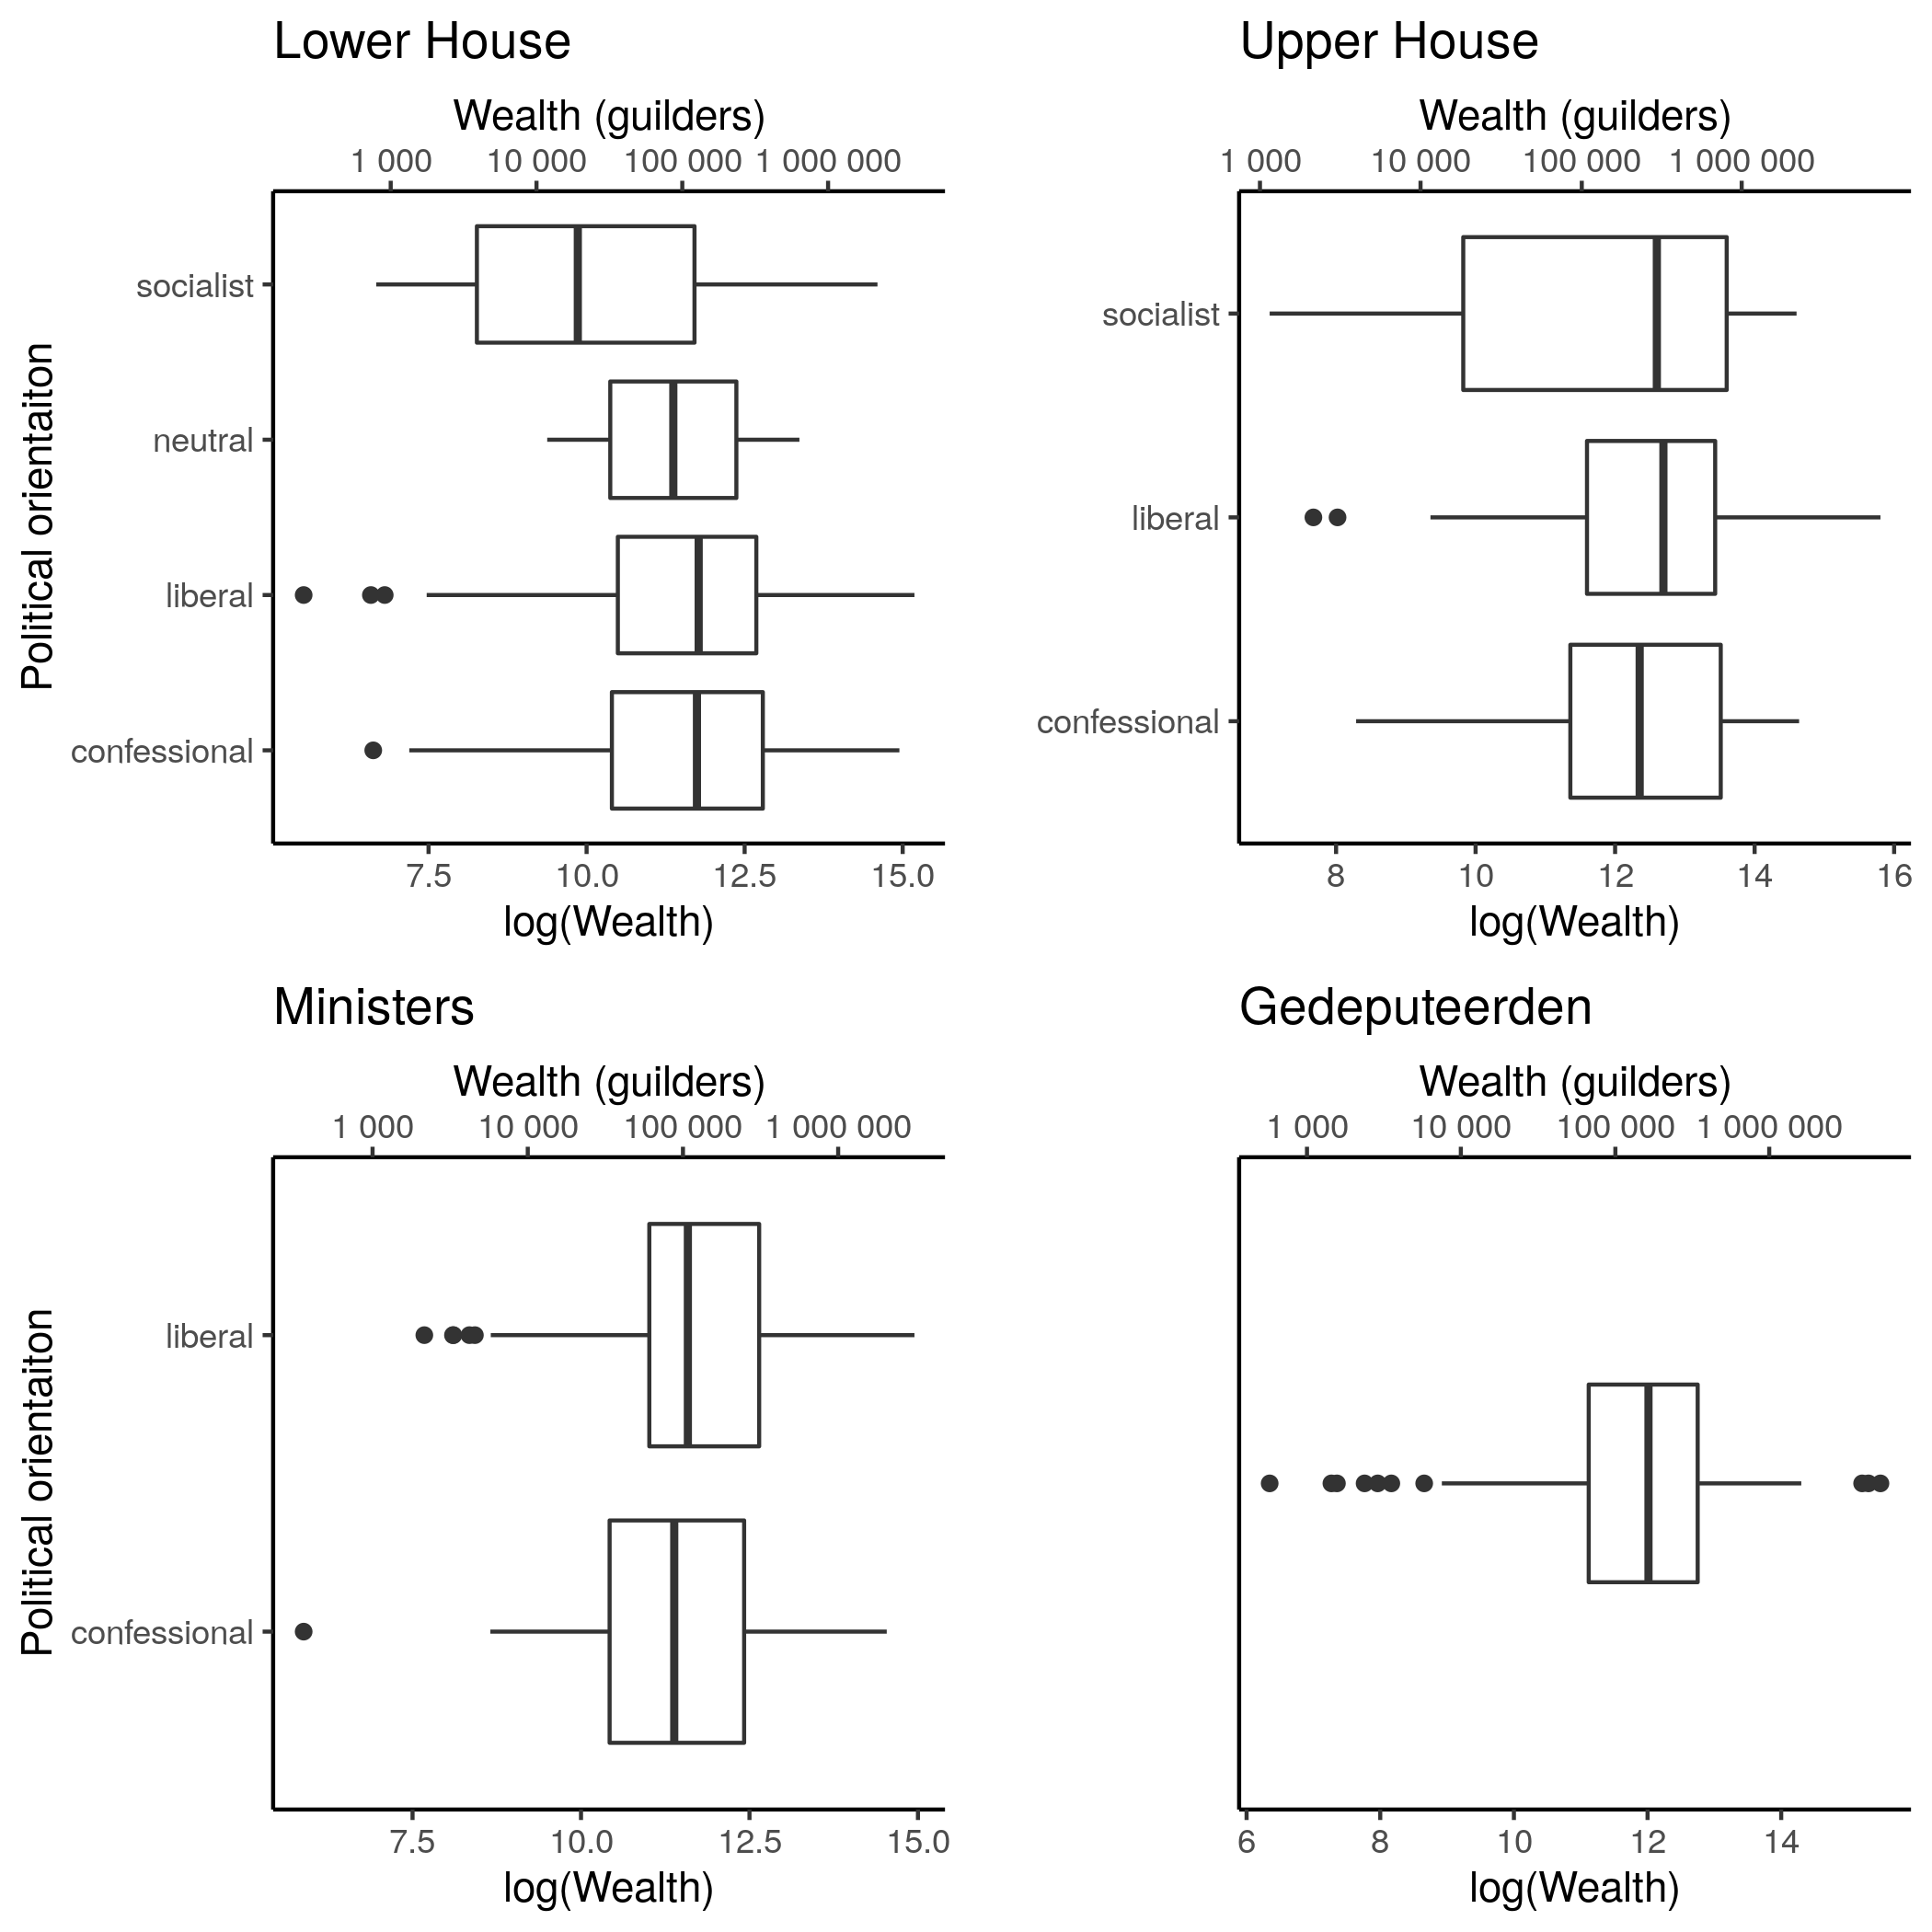
\includegraphics[scale = 0.80]{figures/fig_wealth_function.png}
    \caption{Wealth Distribution According to Function and Party}
    \label{fig:wealthfunction}
\end{figure}

\end{landscape}
\clearpage

% Make table of fig_wealth_function

% latex table generated in R 4.0.2 by xtable 1.8-4 package
% Sun Oct  4 20:31:02 2020
\begin{table}[ht]
\centering
\begin{tabular}{lrrrrrr}
   
\multicolumn{7}{l}{Panel A: Lower House}\\ 
\hline
Political Affiliation & Mean & Median & StdDev & p25 & p75 & n \\\hline

confessional & 264.0 & 96.1 & 441.3 & 17.8 & 326.9 & 165 \\ 
  liberal & 328.1 & 104.2 & 629.1 & 19.5 & 302.8 & 146 \\ 
  neutral & 325.1 & 325.1 & 443.0 & 168.4 & 481.7 & 2 \\ 
  socialist & 201.1 & 13.1 & 496.9 & 3.0 & 112.0 & 23 \\ 
   \hline\\ 
\multicolumn{7}{l}{Panel B: Upper House}\\ 
\hline
Political Affiliation & Mean & Median & StdDev & p25 & p75 & n \\\hline
confessional & 471.6 & 214.4 & 577.3 & 69.1 & 696.7 & 78 \\ 
  liberal & 640.7 & 321.2 & 1052.3 & 99.3 & 681.6 & 82 \\ 
  socialist & 830.3 & 296.0 & 1190.0 & 148.6 & 1244.9 & 3 \\ 
   \hline\\ 
\multicolumn{7}{l}{Panel C: Ministers}\\ 
\hline
Political Affiliation & Mean & Median & StdDev & p25 & p75 & n \\\hline
confessional & 195.8 & 71.7 & 329.1 & 21.2 & 219.1 & 62 \\ 
  liberal & 254.8 & 105.6 & 452.0 & 45.8 & 298.6 & 63 \\ 
  neutral & 26.7 & 24.5 & 23.7 & 8.8 & 42.5 & 7 \\ 
  socialist & 106.6 & 58.3 & 103.7 & 51.9 & 113.0 & 4 \\ 
   \hline\\ 
\multicolumn{7}{l}{Panel D: Regional Executives}\\ 
\hline
Political Affiliation & Mean & Median & StdDev & p25 & p75 & n \\\hline
- & 348.8 & 154.4 & 688.3 & 54.1 & 331.9 & 157 \\ 
   \hline
\multicolumn{7}{l}{}\\
\end{tabular}
\caption{Wealth according to political affiliation ($\cdot 10^{3}$ guilders)} 
\label{tab:wealthfunction}
\end{table}
\clearpage

\begin{landscape}

\begin{figure}
    \centering
    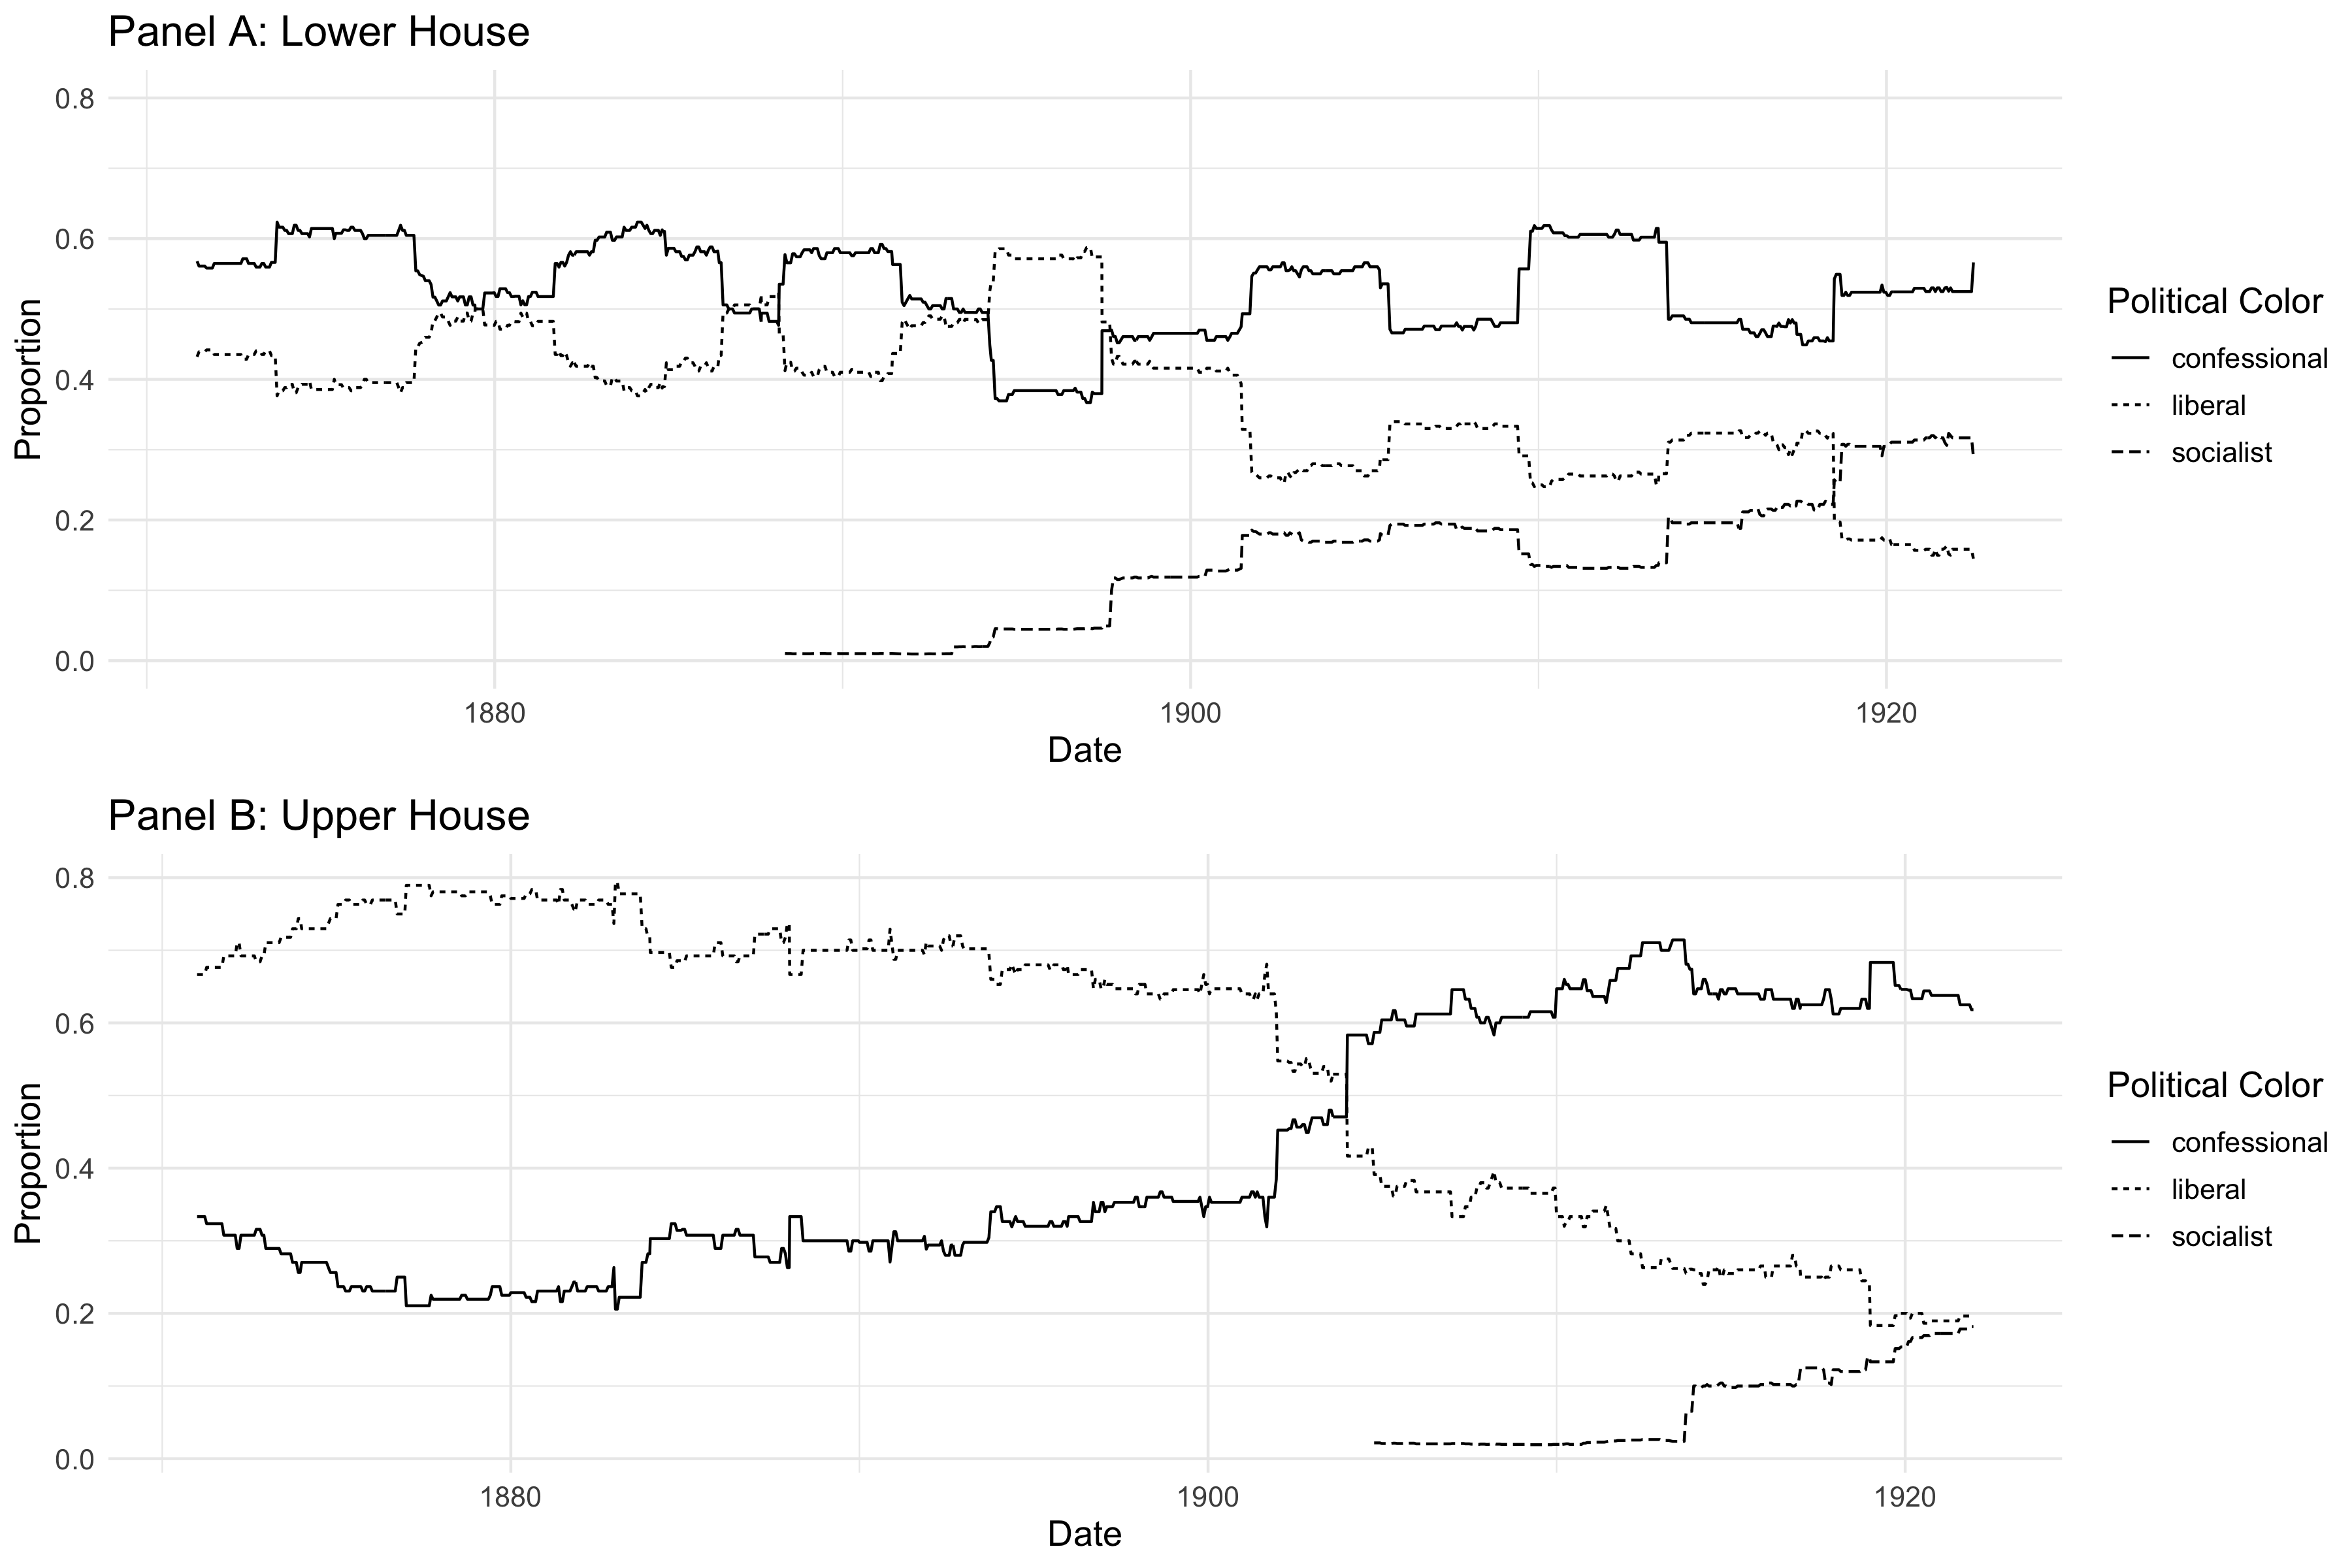
\includegraphics[scale=0.80]{figures/step4comp.png}
    \caption{Political Color of Parliament over Time}
    \label{fig:parltime}
\end{figure}

\end{landscape}
\clearpage

\begin{figure}
    \centering
    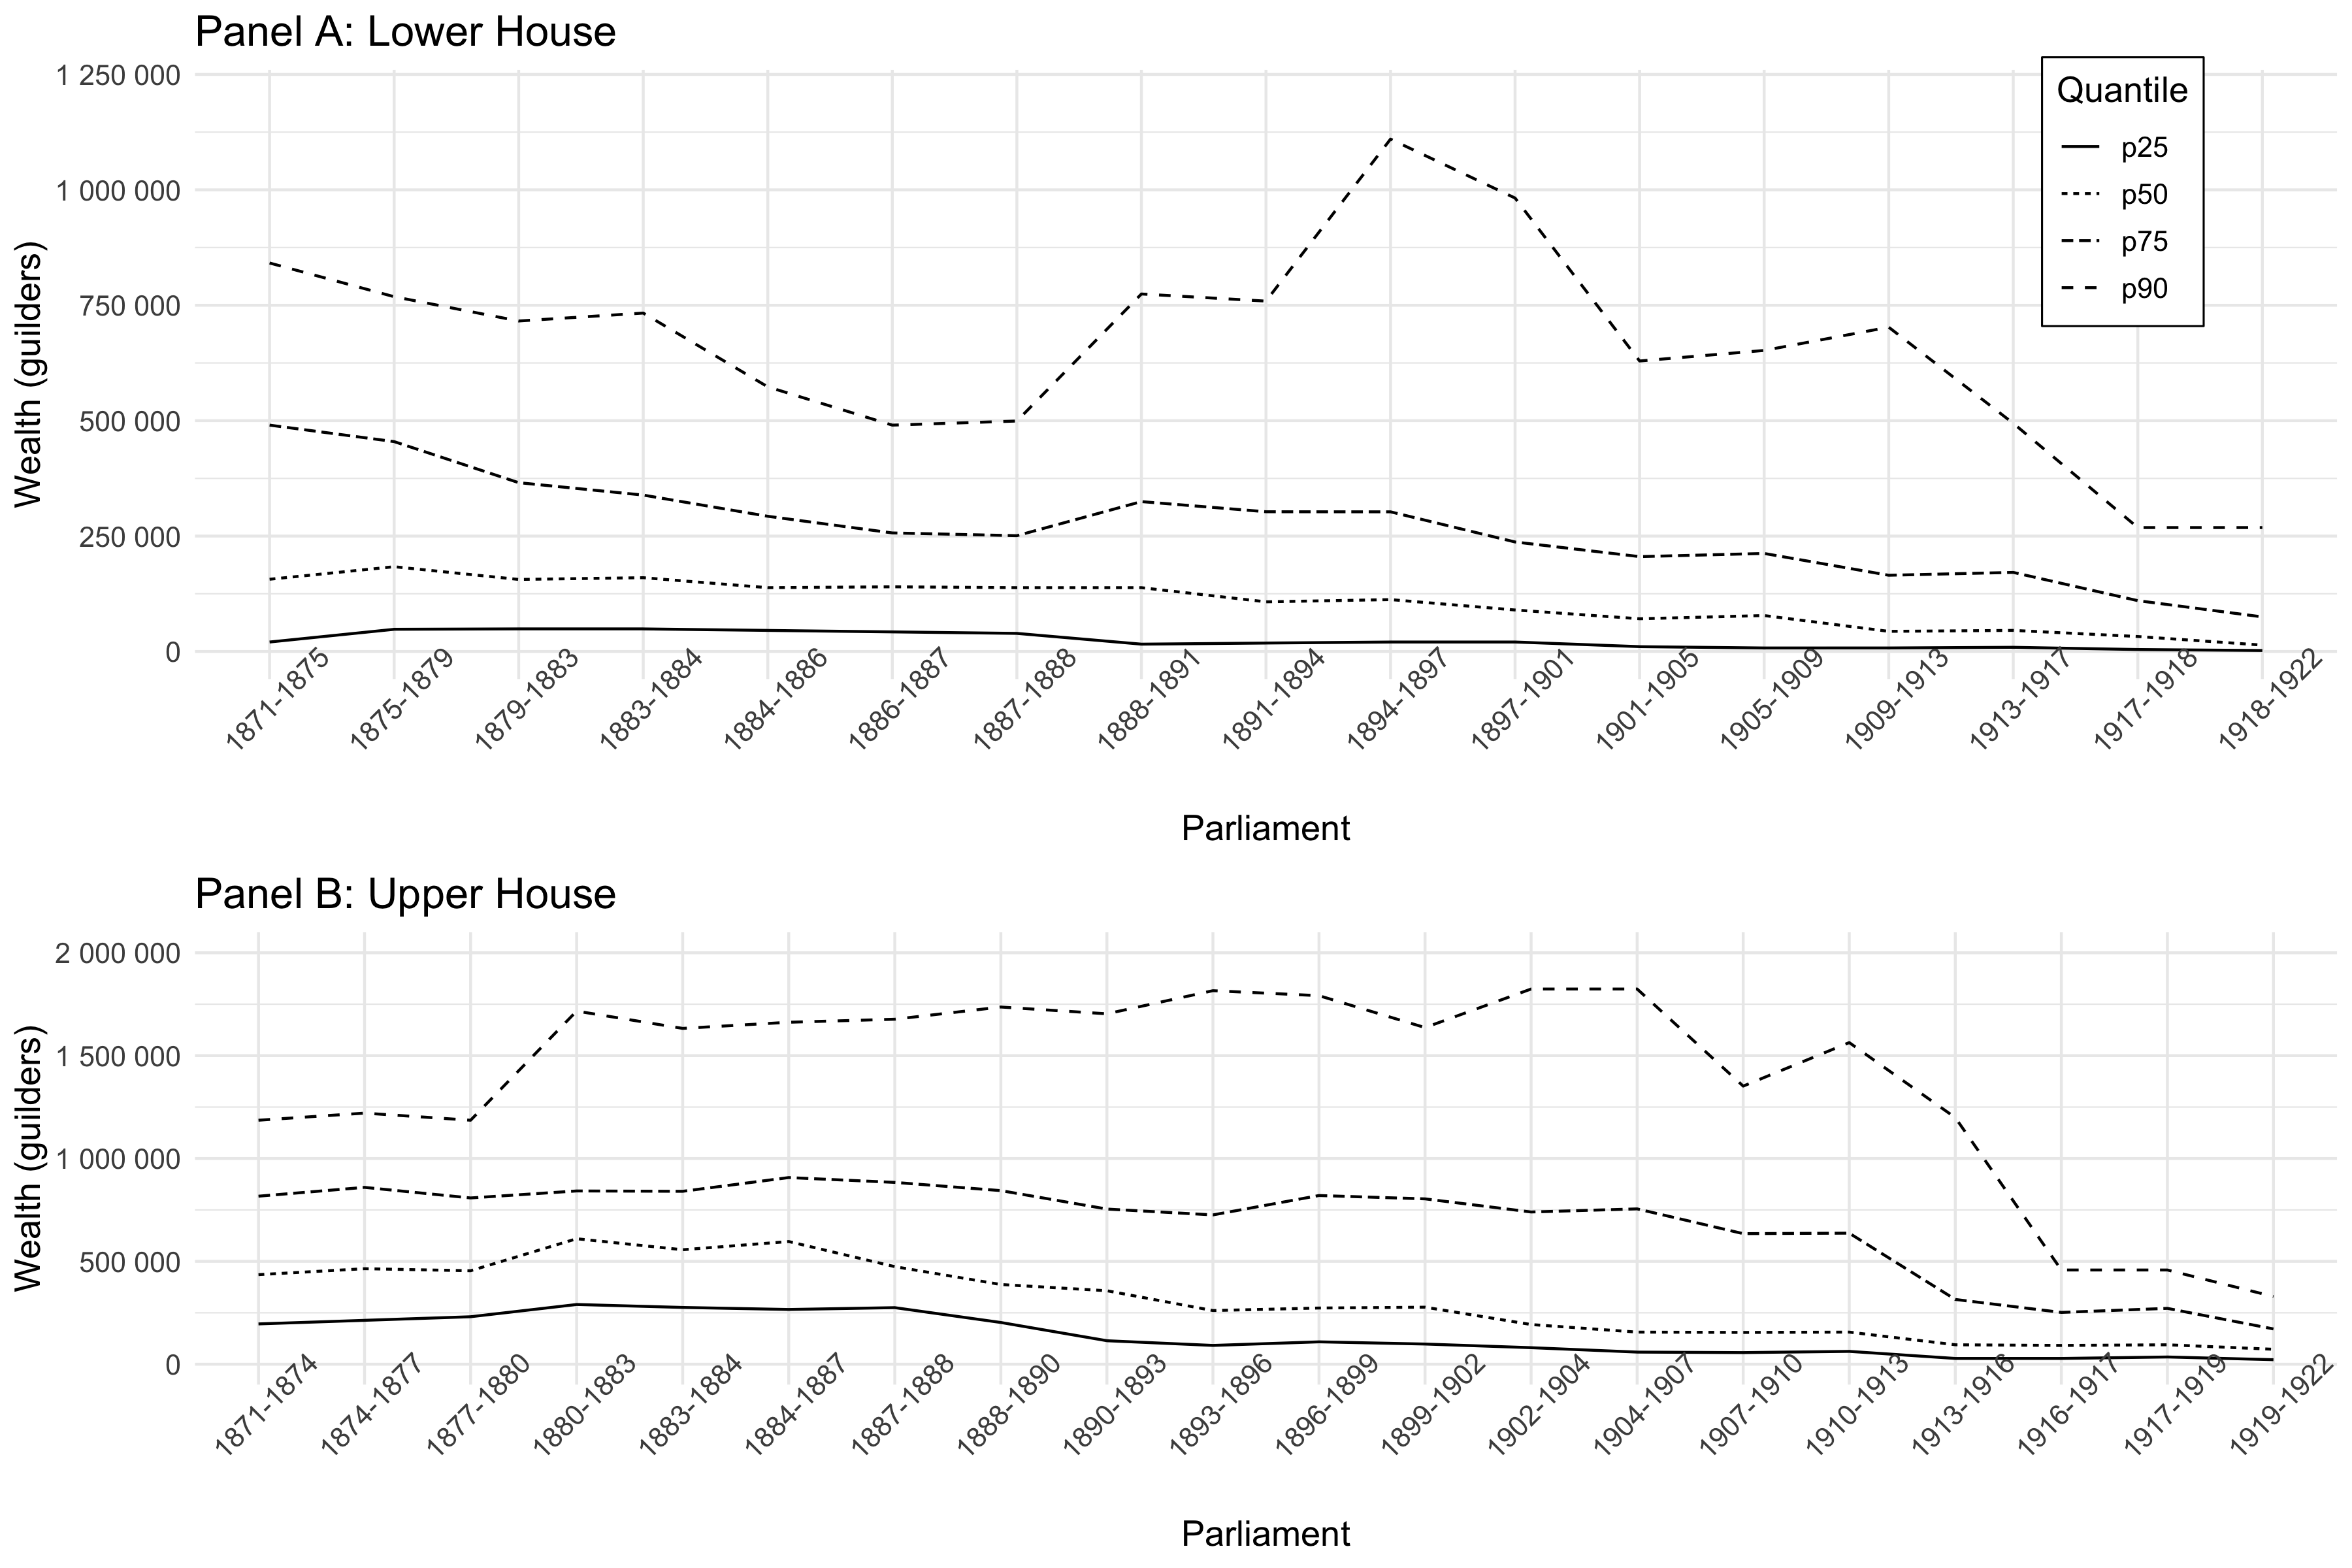
\includegraphics[scale=0.8]{figures/step5fig2wealthperparl.png}
    \caption{Wealth Distribution in Upper and Lower House over Time}
    \label{fig:avgwealthtime}
\end{figure}
\clearpage

\begin{figure}
    \centering
    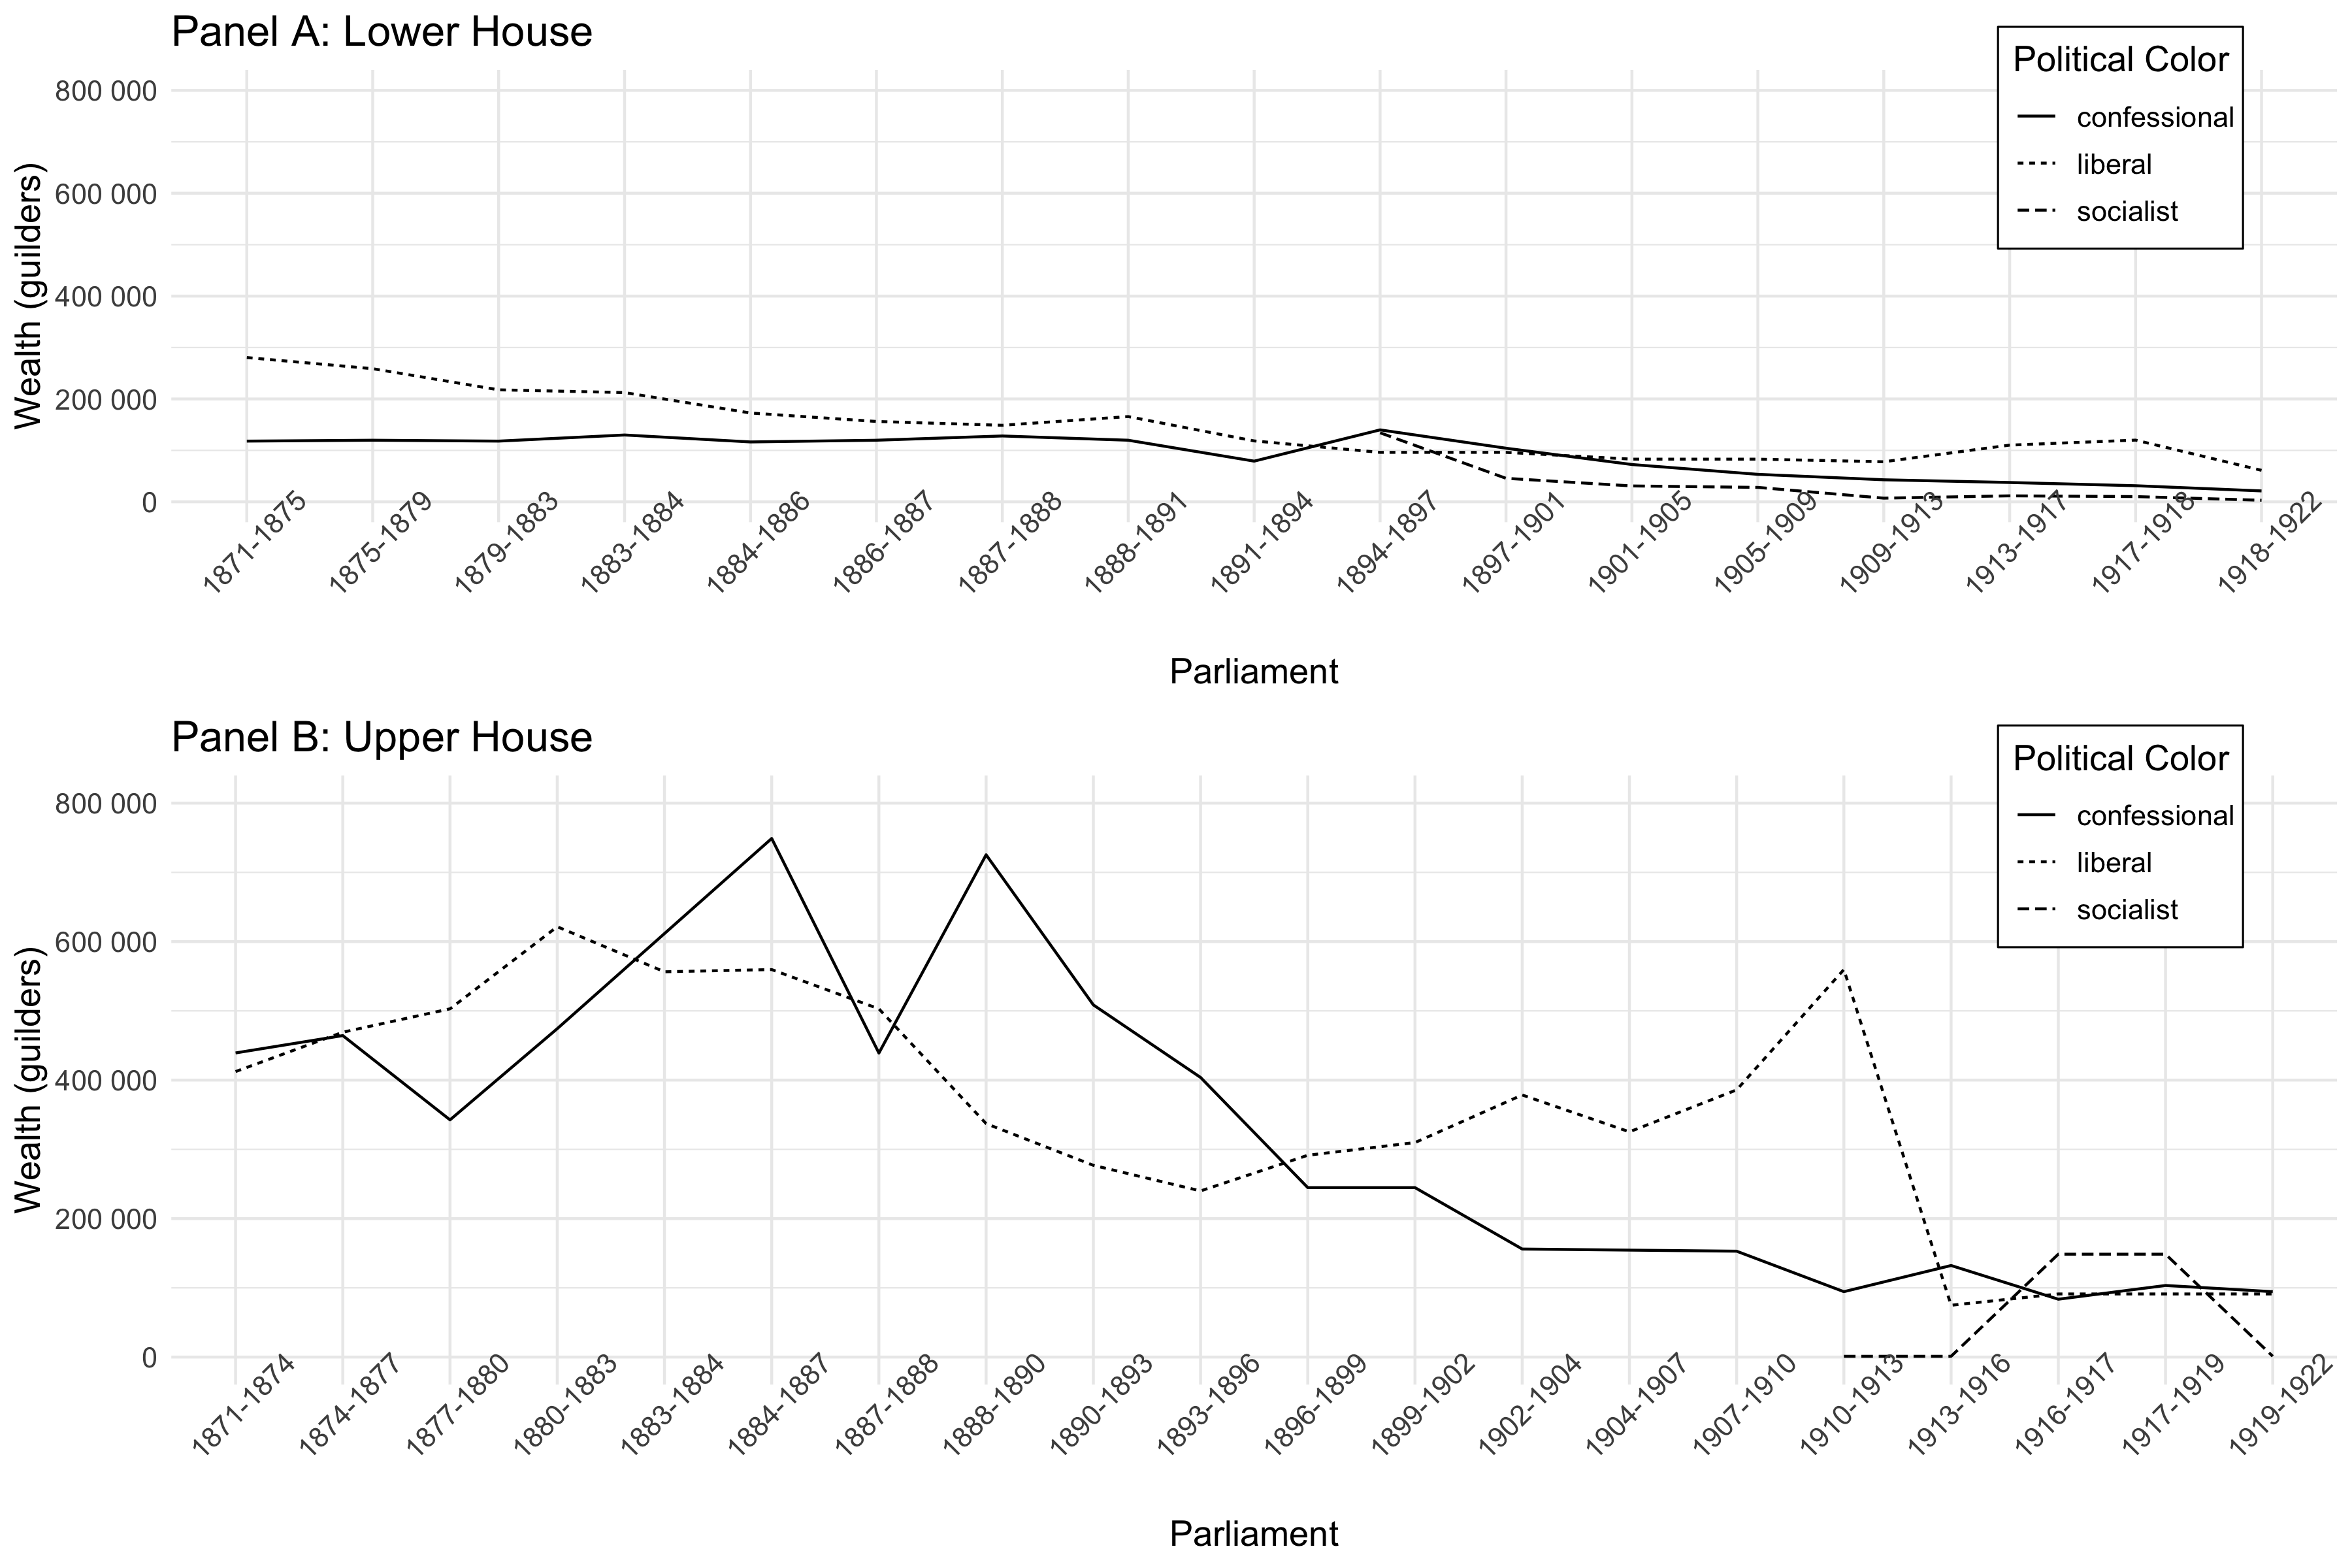
\includegraphics[scale=0.60]{figures/step8fig2wealthperparlperparty.png}
    \caption{Average Wealth per Parliament per Party}
    \label{fig:avgwealthtimeparty}
\end{figure}
\clearpage


% latex table generated in R 3.6.3 by xtable 1.8-4 package
% Wed Aug 19 19:10:42 2020
\begin{table}[ht]
\centering
\begin{tabular}{lrrrrr}
  \hline
House & mean\_re & mean\_shares & mean\_bonds & mean\_misc & n \\ 
  \hline
Lower House & 0.28 & 0.19 & 0.40 & 0.13 & 245 \\ 
  Upper House & 0.44 & 0.19 & 0.30 & 0.07 &  99 \\ 
  Ministers & 0.20 & 0.20 & 0.47 & 0.13 &  96 \\ 
  Provincial Executives & 0.40 & 0.13 & 0.39 & 0.08 & 109 \\ 
   \hline
\end{tabular}
\caption{Before 1900} 
\label{fig:portcomp1_1}
\end{table}


% latex table generated in R 3.6.3 by xtable 1.8-4 package
% Wed Aug 19 19:05:15 2020
\begin{table}[ht]
\centering
\begin{tabular}{lrrrrr}
  \hline
House & mean\_re & mean\_shares & mean\_bonds & mean\_misc & n \\ 
  \hline
Lower House & 0.28 & 0.29 & 0.34 & 0.09 &  73 \\ 
  Upper House & 0.22 & 0.28 & 0.40 & 0.10 &  55 \\ 
  Ministers & 0.14 & 0.33 & 0.39 & 0.14 &  38 \\ 
  Provincial Executives & 0.32 & 0.25 & 0.37 & 0.06 &  45 \\ 
   \hline
\end{tabular}
\caption{After 1900} 
\label{fig:portcomp1_2}
\end{table}


% latex table generated in R 3.6.3 by xtable 1.8-4 package
% Wed Aug 19 19:05:15 2020
\begin{table}[ht]
\centering
\begingroup\small
\begin{tabular}{llrrrrr}
  \hline
House & class & mean\_re & mean\_shares & mean\_bonds & mean\_misc & n \\ 
  \hline
Lower House & confessional & 0.32 & 0.19 & 0.35 & 0.14 & 160 \\ 
  Lower House & liberal & 0.23 & 0.24 & 0.43 & 0.10 & 134 \\ 
  Lower House & neutral & 0.66 & 0.09 & 0.25 & 0.01 &   2 \\ 
  Lower House & socialist & 0.22 & 0.21 & 0.41 & 0.16 &  22 \\ 
  Upper House & confessional & 0.35 & 0.19 & 0.34 & 0.11 &  72 \\ 
  Upper House & liberal & 0.37 & 0.25 & 0.33 & 0.05 &  79 \\ 
  Upper House & socialist & 0.52 & 0.10 & 0.29 & 0.09 &   3 \\ 
  Ministers & confessional & 0.24 & 0.20 & 0.42 & 0.14 &  61 \\ 
  Ministers & liberal & 0.14 & 0.26 & 0.48 & 0.13 &  63 \\ 
  Ministers & neutral & 0.10 & 0.24 & 0.53 & 0.13 &   6 \\ 
  Ministers & socialist & 0.21 & 0.36 & 0.38 & 0.06 &   4 \\ 
   \hline
\end{tabular}
\endgroup
\caption{Portfolio Composition according to Political Color} 
\label{fig:portcomp2}
\end{table}

\clearpage

\begin{landscape}
% latex table generated in R 3.6.3 by xtable 1.8-4 package
% Wed Aug 19 10:37:22 2020
\begin{table}[ht]
\centering
\begin{tabular}{lrrrrr}
  \hline
Government & Mean & Median & SD & N & WealthPM \\ 
  \hline
Thorbecke III & 178154 & 95554 & 201112 & 7 &  \\ 
  De Vries/Fransen van de Putte & 81432 & 60689 & 76062 & 7 &  \\ 
  Heemskerk/Van Lynden van Sandenburg & 291140 & 220192 & 280563 & 9 & 623456 \\ 
  Kappeyne van de Coppello & 723896 & 446626 & 942720 & 10 & 485686 \\ 
  Van Lynden van Sandenburg & 220697 & 160340 & 237914 & 10 & 748926 \\ 
  Heemskerk Azn. & 152602 & 57739 & 190782 & 13 & 623456 \\ 
  Mackay & 92411 & 81022 & 88781 & 8 & 246825 \\ 
  Van Tienhoven & 406770 & 233273 & 568110 & 6 & 365691 \\ 
  Röell & 158083 & 55433 & 207810 & 7 & 559626 \\ 
  Pierson & 98497 & 100291 & 55039 & 7 &  \\ 
  Kuyper & 317188 & 53429 & 770428 & 7 & 112404 \\ 
  De Meester & 156490 & 63356 & 244954 & 9 & 36111 \\ 
  Heemskerk & 62610 & 21440 & 108579 & 10 &  \\ 
  Cort van der Linden & 109307 & 97571 & 66149 & 8 & 100291 \\ 
  Ruijs de Beerenbrouck I & 80876 & 24459 & 145993 & 7 &  \\ 
   \hline
\end{tabular}
\caption{Average Wealth of Governments} 
\end{table}

\clearpage


\begin{figure}
    \centering
    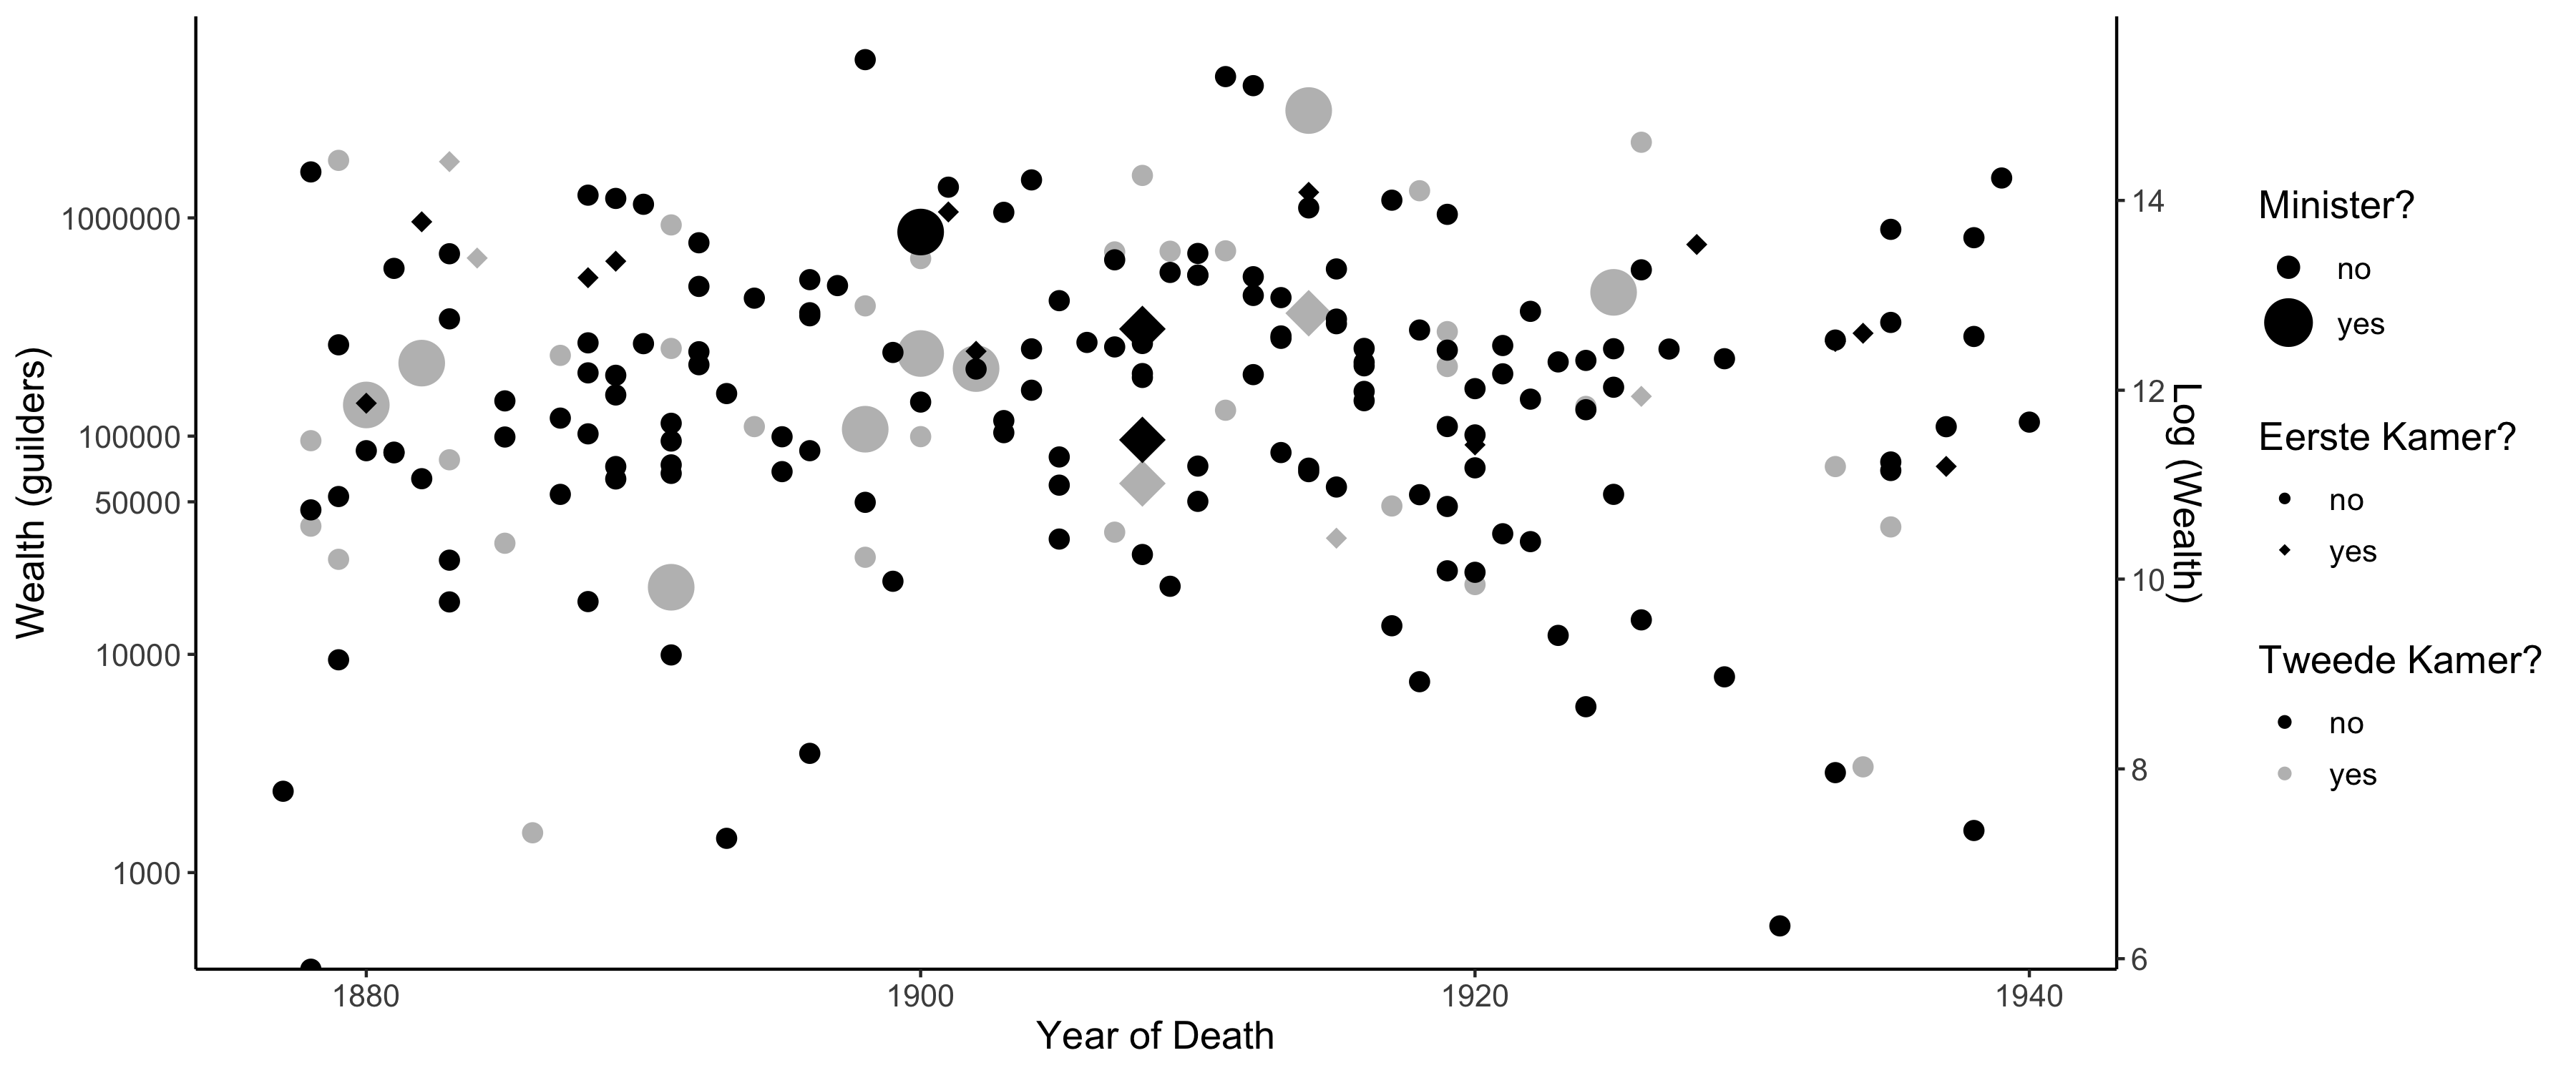
\includegraphics[scale = 0.80]{figures/wealth_dep.png}
    \caption{Wealth of Provincial Executives over Time}
    \label{fig:avgwealthprovexec}
\end{figure}
\clearpage
\end{landscape}

% latex table generated in R 4.0.2 by xtable 1.8-4 package
% Mon Oct  5 02:26:50 2020
\begin{table}[ht]
\centering
\begingroup\footnotesize
\begin{tabular}{lrrrrrr}
   
\multicolumn{7}{l}{Panel A:Lower House}\\ 
\hline
parliament & min & p25 & p75 & max & gini & gini2 \\\hline

1871-1875 & 1.33 & 28.7 & 521.8 & 1834.6 & 0.606 & 0.598 \\ 
  1875-1879 & 1.33 & 61.8 & 469.7 & 1834.6 & 0.589 & 0.571 \\ 
  1879-1883 & 1.33 & 63.5 & 424.9 & 3103.7 & 0.602 & 0.572 \\ 
  1883-1884 & 1.33 & 65.2 & 413.8 & 3103.7 & 0.596 & 0.557 \\ 
  1884-1886 & 0.90 & 65.5 & 307.6 & 1178.6 & 0.528 & 0.514 \\ 
  1886-1887 & 0.90 & 84.3 & 269.9 & 1331.8 & 0.523 & 0.499 \\ 
  1887-1888 & 0.90 & 79.9 & 270.1 & 1565.3 & 0.542 & 0.512 \\ 
  1888-1891 & 0.75 & 58.8 & 393.7 & 3938.4 & 0.655 & 0.621 \\ 
  1891-1894 & 0.75 & 35.0 & 324.1 & 3938.4 & 0.692 & 0.661 \\ 
  1894-1897 & 0.75 & 34.1 & 302.9 & 3938.4 & 0.741 & 0.719 \\ 
  1897-1901 & 0.25 & 23.5 & 287.6 & 3938.4 & 0.755 & 0.736 \\ 
  1901-1905 & 0.73 & 23.5 & 277.2 & 2221.3 & 0.715 & 0.699 \\ 
  1905-1909 & 0.73 & 20.0 & 258.1 & 2221.3 & 0.721 & 0.715 \\ 
  1909-1913 & 0.73 & 15.1 & 181.6 & 2221.3 & 0.770 & 0.761 \\ 
  1913-1917 & 0.73 & 13.1 & 212.4 & 2221.3 & 0.725 & 0.691 \\ 
  1917-1918 & 0.73 & 9.8 & 133.2 & 2221.3 & 0.744 & 0.620 \\ 
  1918-1922 & 1.00 & 8.4 & 96.1 & 638.3 & 0.703 & 0.679 \\ 
   \hline\\ 
\multicolumn{7}{l}{Panel B:Upper House}\\ 
\hline
parliament & min & p25 & p75 & max & gini & gini2 \\\hline
1871-1874 & 3.04 & 244.6 & 821.1 & 1743.0 & 0.458 & 0.444 \\ 
  1874-1877 & 3.04 & 258.4 & 880.5 & 3067.1 & 0.487 & 0.445 \\ 
  1877-1880 & 11.53 & 272.1 & 812.5 & 3067.1 & 0.459 & 0.415 \\ 
  1880-1883 & 11.53 & 303.3 & 843.9 & 3067.1 & 0.445 & 0.410 \\ 
  1883-1884 & 11.53 & 281.4 & 842.2 & 1966.1 & 0.415 & 0.402 \\ 
  1884-1887 & 48.10 & 275.0 & 912.3 & 1966.1 & 0.418 & 0.409 \\ 
  1887-1888 & 48.10 & 276.9 & 903.0 & 2057.1 & 0.436 & 0.424 \\ 
  1888-1890 & 19.21 & 206.8 & 845.5 & 2057.1 & 0.499 & 0.493 \\ 
  1890-1893 & 19.21 & 123.0 & 789.8 & 2057.1 & 0.542 & 0.537 \\ 
  1893-1896 & 19.21 & 105.6 & 766.4 & 7303.5 & 0.654 & 0.574 \\ 
  1896-1899 & 39.49 & 122.8 & 832.8 & 7303.5 & 0.661 & 0.603 \\ 
  1899-1902 & 39.49 & 117.0 & 826.4 & 7303.5 & 0.656 & 0.596 \\ 
  1902-1904 & 4.53 & 90.9 & 743.7 & 7303.5 & 0.707 & 0.653 \\ 
  1904-1907 & 2.15 & 67.1 & 817.1 & 4749.5 & 0.680 & 0.646 \\ 
  1907-1910 & 2.15 & 68.2 & 641.7 & 2364.5 & 0.647 & 0.639 \\ 
  1910-1913 & 1.15 & 68.2 & 641.7 & 2364.5 & 0.654 & 0.647 \\ 
  1913-1916 & 1.15 & 33.4 & 335.4 & 2275.6 & 0.729 & 0.724 \\ 
  1916-1917 & 1.15 & 33.4 & 262.9 & 2193.8 & 0.731 & 0.692 \\ 
  1917-1919 & 1.15 & 39.1 & 277.7 & 2193.8 & 0.706 & 0.661 \\ 
  1919-1922 & 1.15 & 25.0 & 196.7 & 702.4 & 0.590 & 0.544 \\ 
   \hline
\multicolumn{7}{l}{}\\
\end{tabular}
\endgroup
\caption{Wealth Distribution over Time (1000 Guilders)} 
\label{tab:ginicoef}
\end{table}

\end{document}
